\documentclass[a4paper,fleqn]{cas-sc}

\usepackage{booktabs}
\usepackage{multirow}
\usepackage{array}
\usepackage{graphicx}
\usepackage{amssymb}
\usepackage{amsmath}
\usepackage{textcomp}
\usepackage{float}
\usepackage{hyperref}
\usepackage[capitalize,noabbrev]{cleveref}
\usepackage{threeparttable}
\usepackage[tableposition=top]{caption}
\usepackage{subcaption}
\usepackage{bm}
\usepackage{xcolor}
\usepackage{colortbl}
\usepackage{algorithm}
\usepackage{algorithmic}
\usepackage[numbers]{natbib}

\hypersetup{
  colorlinks=true,
  linkcolor=blue,
  citecolor=blue,
  urlcolor=blue
}

\graphicspath{{figures/}}

\makeatletter
\renewcommand{\dbltopfraction}{0.9}
\renewcommand{\dblfloatpagefraction}{0.9}
\makeatother

\newcommand{\method}{SharedClass}
\newcommand{\dataset}{SCB5}

\begin{document}
\let\WriteBookmarks\relax
\def\floatpagepagefraction{1}
\def\textpagefraction{.001}

\shorttitle{Shared Class-Neighborhood Geometry}

\shortauthors{Zhang and Ma}

\title[mode=title]{Shared Class-Neighborhood Geometry: A Candidate Mechanism for Why CLIP Predicts MLLM Difficulty}

\author[1]{Lizhuo Zhang}[orcid=0009-0004-0749-3239]
\cormark[1]
\ead{zhanglizhuo@hunau.edu.cn}
\credit{Conceptualization, Methodology, Software, Validation, Formal analysis, Investigation, Writing---original draft, Writing---review and editing, Supervision}

\author[2]{Yan Ma}[orcid=0009-0002-5071-0054]
\ead{mayan@csust.edu.cn}
\credit{Conceptualization, Investigation, Writing---review and editing}

\affiliation[1]{organization={School of Information and Intelligence, Hunan Agricultural University},
            city={Changsha},
            postcode={410128},
            country={China}}

\affiliation[2]{organization={School of Foreign Studies, Changsha University of Science and Technology},
            city={Changsha},
            postcode={410114},
            country={China}}

\cortext[1]{Corresponding author.}

\begin{highlights}
\item Independently trained vision encoders converge to shared class geometry
\item An ImageNet-only ResNet-50 recovers this geometry, weakening data-overlap accounts
\item Shared structure is strongest at class prototypes, not patches (adapter R2 <= 0.21)
\item Mediation quantifies the shared-difficulty component of the CLIP-MLLM correlation
\item Preregistered encoder intervention yields a boundary; prompts repair CLIP's failures
\end{highlights}

\begin{abstract}
Vision encoders trained on diverse large-scale data, with different architectures and objectives, exhibit a broadly shared \emph{class-neighborhood geometry}: a statistically shared structure in which class prototypes are relatively close in representation space. A behavioral consequence of this shared geometry is that CLIP zero-shot accuracy, computable in minutes, forecasts the per-class difficulty of multimodal language models (MLLMs) one to nearly two orders of magnitude larger. Why, then, does one system's per-class difficulty replicate in the other? We test the candidate mechanism (shared class-neighborhood geometry) across twelve MLLMs from four vision-encoder families, seven vision encoders, and three domains.

Five lines of evidence support this account. First, the correlation is not an artifact of shared encoder weights: MLLMs with encoders different from CLIP (SigLIP group $\rho=0.716$, QwenViT group $\rho=0.669$) retain strong correlations, and family-level tests show systematic differences across encoder groups, providing evidence against the shared-encoder interpretation. Second, class-centroid similarity matrices agree strongly across independently trained encoders (Mantel $\rho=0.90$--$0.98$ on 8 classes), a pattern that extends to 40 and 102 classes; a supervised ImageNet-1k-only ResNet-50 recovers the same geometry ($\rho=0.93$--$0.98$), while a DINOv2 encoder trained with more data and more corpus overlap agrees more weakly, weakening a data-overlap account. Third, the shared structure localizes to the class-neighborhood level: an adapter explains at most 21\% of per-patch variance, whereas class-centroid geometry agrees at $\rho=0.90$--$0.96$. Fourth, bootstrap mediation quantifies a substantial shared-difficulty component of the CLIP--MLLM correlation on Stanford40, with small residual direct effects. Fifth, CLIP's most striking per-class failures are resolved by prompt engineering (e.g., 0\%$\rightarrow$100\%), indicating that they reflect text--image alignment rather than absence of useful visual information.

Together these results are consistent with shared class-neighborhood geometry as the parsimonious account linking lightweight CLIP evaluation to MLLM difficulty, though they do not establish it definitively. The analyses are observational; a preregistered causal intervention (a frozen language model paired with equal-budget projectors over four swapped vision encoders) yielded a boundary rather than a confirmation: downstream difficulty did not follow encoder-geometry similarity, and the causal link remains open.
\end{abstract}

\begin{keywords}
representation similarity \sep class geometry \sep CLIP \sep multimodal language models \sep zero-shot evaluation \sep visual anchoring
\end{keywords}

\maketitle

\section{Introduction}
\label{sec:intro}

The per-class zero-shot accuracy of CLIP (Vision Transformer, $\sim$428M parameters), a model released in 2021 with a simple contrastive objective, predicts the per-class accuracy of large multimodal language models (MLLMs) that are one to nearly two orders of magnitude larger and trained with autoregressive language modeling \cite{ma2025anchorscore}. On a classroom behavior dataset, this correlation reaches Spearman $\rho\approx0.77$, with consistent replication on human action recognition ($\rho=0.82$). The practical value is clear: CLIP evaluation takes 3 minutes on a single GPU, while evaluating a single MLLM on the same benchmark requires hours of GPU time.

This finding presents a paradox. CLIP and modern MLLMs differ in nearly every design dimension: architecture (ViT vs. hybrid vision-language transformers), training objective (contrastive vs. next-token prediction), parameter count (0.4B vs. 7B--35B), and training data (WIT-400M vs. Internet-scale multimodal corpora). If these models are so different, why do their per-class difficulty rankings align?

Four hypotheses can explain this correlation:

\begin{enumerate}
  \item \textbf{Shared encoder hypothesis (H1):} The correlation is trivial: MLLMs use CLIP as their vision encoder, so shared visual features produce shared limitations.
  \item \textbf{Shared data hypothesis (H2):} Overlapping training data causes both models to find the same classes easy or hard.
  \item \textbf{Shared class-neighborhood geometry hypothesis (H3, ours):} Vision encoders trained on diverse large-scale data independently converge to similar class-neighborhood geometry, providing a structural correlate of shared per-class difficulty.
  \item \textbf{Raw image difficulty hypothesis (H4):} The correlation reflects intrinsic image-level difficulty (low quality, ambiguous, or atypical instances) rather than any encoder-side property: every model simply fails on the same hard images, producing the appearance of shared per-class difficulty without any shared representation.
\end{enumerate}

We define \emph{shared class-neighborhood geometry} as the phenomenon that independently trained vision encoders learn highly similar pairwise relationships among semantic classes: two classes that are close in one encoder's feature space will be close in every encoder's space. We further distinguish three levels of analysis: \emph{class-neighborhood geometry} (the pairwise similarity structure of class centroids in a feature space), \emph{class confusability} (which class pairs are hard to tell apart, the behavioral translation of geometry), and \emph{per-class difficulty} (the observable outcome, e.g., classification accuracy). This paper measures geometry directly (CKA, Mantel tests, \S\ref{sec:geometry}) and treats the further step from geometry to confusability as a defined behavioral translation rather than a separately measured link; an empirical within-MLLM test of this link is reported in Supplement \S2 and yields a null result ($\rho=+0.09$, $p=0.64$), supporting the geometry framing. The chain from geometry to difficulty is not automatic (a model may misclassify a class for semantic alignment reasons rather than geometric ones, \S\ref{sec:prompt}), and each link requires separate evidence. H2 and H4 are distinct non-geometric alternatives (one about overlapping training corpora, the other about the images themselves), and each is addressed by a dedicated control below (\S\ref{sec:geometry}, \S\ref{sec:prompt}).

Distinguishing these hypotheses is not merely an academic exercise. If the shared-encoder hypothesis were true, the diagnostic power of AnchorScore (the per-class CLIP zero-shot accuracy used as the predictor throughout this paper) would be limited to CLIP-based MLLMs and would diminish as models adopt custom encoders. If shared class-neighborhood geometry is the mechanism, AnchorScore measures a fundamental property of visual representations that transcends any specific model: a claim with broad implications for model evaluation, representation learning, and our understanding of Internet-scale vision.

Previous work has not resolved this question. While several studies observe that different vision models share a ``partial consensus'' on difficulty \cite{geirhos2021partial} and learn similar feature spaces under Internet-scale training \cite{kornblith2019similarity}, none has established \emph{why} this consensus arises or whether it fully explains the CLIP--MLLM correlation.

This paper systematically distinguishes these hypotheses through five lines of evidence, organized into three strands that map onto the proposed chain of \Cref{fig:overview}. The \emph{mechanism strand} first establishes the phenomenon across datasets and twelve MLLMs spanning four vision-encoder families (\S\ref{sec:phenomenon}), then provides evidence against the shared-encoder artifact: MLLMs whose encoders differ from CLIP (SigLIP group $\rho=0.716$; QwenViT group $\rho=0.669$) retain strong correlations. Family-level tests (Kruskal--Wallis $p=0.030$) show systematic differences across encoder groups, providing evidence against the interpretation that the effect is confined to CLIP-based MLLMs (\S\ref{sec:ruleout}). The \emph{cross-domain strand} tests the geometric prediction directly and out-of-sample: class-centroid neighborhood matrices agree strongly across independently trained encoders (Mantel $\rho=0.90$--$0.98$; geometry-statistic bootstrap CI $[0.74,0.87]$ at 40 classes; the behavioral-correlation CI is reported in \S\ref{sec:phenomenon}), the agreement generalizes from 8 to 102 fine-grained classes and from fully public ImageNet-1k training to Internet-scale corpora, and bootstrap mediation quantifies a substantial shared-difficulty component of the CLIP--MLLM correlation (\S\ref{sec:geometry}, \S\ref{sec:mediation}). The \emph{transfer strand} tests behavioral alignment: CLIP's most striking per-class failures (resolvable by prompt engineering, 0\%$\rightarrow$100\%) show the vision encoder perceives these concepts but maps them to incorrect text representations, indicating that the difficulty signal is not driven by absent visual features alone (\S\ref{sec:prompt}).

\begin{figure*}[t]
\centering
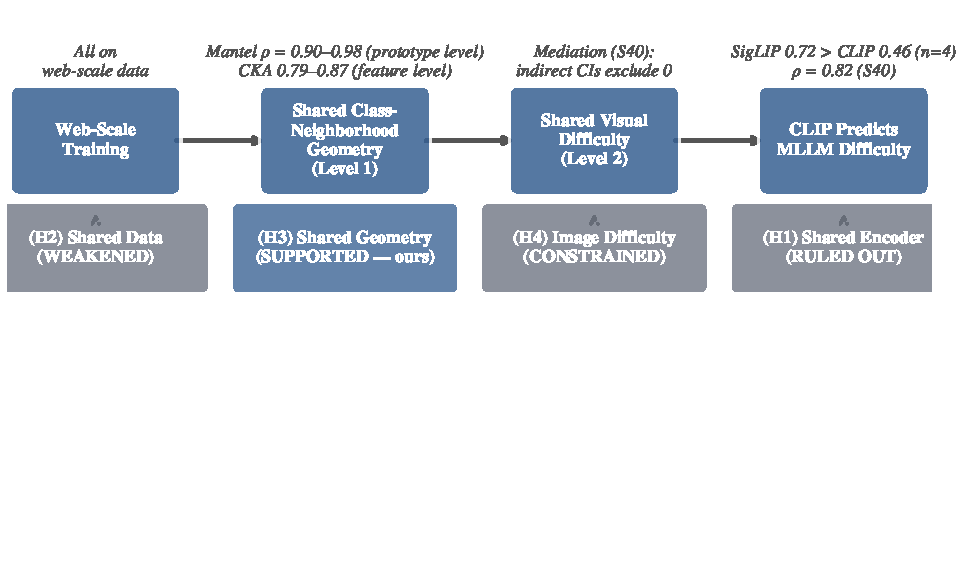
\includegraphics[width=\textwidth]{fig1_phenomenon_overview.pdf}
\caption{The hypothesized two-level model. Diverse Internet-scale training drives independently trained vision encoders to converge to a shared class-neighborhood geometry (Level~1, H3), which is associated with shared per-class visual difficulty (Level~2); AnchorScore correlates with MLLM difficulty insofar as it captures this shared geometry. Above each stage, italic text gives the supporting evidence. Dashed arrows indicate the specific link each competing hypothesis challenges (H2 attacks training-to-geometry, where the solid arrow marks H3 as the supported account; H4 attacks geometry-to-difficulty; H1 attacks difficulty-to-prediction). Downstream error patterns are additionally shaped by the factors summarized in the bottom band; arrows denote observational associations, not causal pathways.}
\label{fig:overview}
\end{figure*}

\section{Related Work}
\label{sec:related}

Three lines of research touch on the question, but none addresses the mechanism linking CLIP's zero-shot accuracy to MLLM difficulty.

\paragraph{Predicting MLLM Performance.}
The visual-anchoring concept behind this diagnostic originates in the analysis of multimodal pseudo-label reliability by Ma and Zhang \cite{la}; the AnchorScore diagnostic itself was introduced by Ma and Zhang \cite{ma2025anchorscore} as a predictor of MLLM per-class accuracy, demonstrating robust correlation across datasets and MLLM families. Existing work develops instruction-tuned MLLMs such as LLaVA \cite{liu2023visual}, but none explains \emph{why} a frozen CLIP model, released in 2021, predicts the per-class accuracy of models nearly two orders of magnitude larger.

\paragraph{Representation Similarity.}
Kornblith et al. \cite{kornblith2019similarity} showed that CKA between models increases with training data scale; the field-standard survey of functional and representational similarity measures is Klabunde et al.~\cite{klabunde2023similarity}. Kriegeskorte et al. \cite{kriegeskorte2008representational} formalized representational similarity analysis (RSA) for comparing neural representations. Huh et al.~\cite{huh2024platonic} go furthest, arguing that representations across modalities are converging toward a shared statistical model of reality (the ``Platonic representation''); recent re-examinations caution that standard similarity metrics can be inflated by network scale and propose permutation-based null-calibration \cite{groger2026aristotelian}. Complementary analyses show that internal representation structure depends on architecture and training procedure (ViT vs.\ CNN \cite{raghu2021vitcnn}), that transfer learning reuses low-level feature statistics rather than high-level semantics alone \cite{neyshabur2020transfer}, that latent spaces of independently trained models can be aligned zero-shot without anchors via relative representations \cite{moschella2022relative}, and that the training objective---rather than shared data---drives the consistency of representational similarity across datasets \cite{ciernik2024objective}. These works establish \emph{that} representations converge; they do not test whether the convergence explains a specific cross-model behavioral regularity such as the CLIP--MLLM per-class correlation, nor do they quantify how much of that regularity the shared geometry accounts for; that is the empirical question addressed here.

\paragraph{Visual Confusability.}
Geirhos et al. \cite{geirhos2021partial} showed that vision models share a ``partial consensus'' on which classes are difficult, quantified by the error-consistency metric of Geirhos et al.~\cite{geirhos2020error}; similarly, model similarity is known to translate into shared error structure: Mania et al.~\cite{mania2019model} showed that similar models make similar mistakes, with consequences for test-set reuse. Prior work on attribute- and part-based action recognition \cite{yao2011stanford40} addresses class confusability within a single model. At the instance level, training-dynamics analyses distinguish easy, ambiguous, and hard examples within a single model \cite{swayamdipta2020cartography}. However, no prior work proposes that this confusability is \emph{shared across independently trained encoders}, or that it underlies the CLIP--MLLM correlation.

\paragraph{The Mechanism Gap.}
Representations converge and CLIP predicts MLLM difficulty, but the specific link, that shared class-neighborhood geometry underlies this behavioral correlation and that the simpler shared-encoder account is wrong, has not been quantified or falsification-tested. The present paper provides that test: we measure the geometry directly, quantify the fraction of the correlation mediated by shared difficulty, and empirically provide evidence against the shared-encoder explanation.

\section{Experimental Setup}
\label{sec:setup}

\subsection{Datasets}

We evaluate on three datasets: two with MLLM annotations (\textbf{SCB5} and \textbf{Stanford40 Actions}) and one geometric-only benchmark (\textbf{Flowers102}). \textbf{SCB5} (Smart Classroom Behavior v5) \cite{la} is a classroom behavior benchmark comprising three sub-datasets whose classes we pool for added statistical power: \emph{TeacherBehavior} (8 classes: guide, answer, On-stage interaction, blackboard-writing, teacher, stand, screen, blackBoard; note that \texttt{blackboard-writing} denotes the act of writing on the board while \texttt{blackBoard} denotes the board as a visual object; they are distinct classes with disjoint image sets but visually related content, which the prompt experiment of \S\ref{sec:prompt} addresses), \emph{HandriseReadWrite} (3 classes), and \emph{BowTurnHead} (2 classes), giving 13 classes in total (20 images/class for CKA feature analysis, 50 images/class for class similarity matrices). The main geometric analysis (CKA, class similarity matrices) uses the 8 TeacherBehavior classes, where all seven encoders were evaluated; the mediation analysis (\S\ref{sec:mediation}) pools all 13 classes to maximize power. \textbf{Stanford40 Actions} \cite{yao2011stanford40} contains 40 human action classes (9,532 images) and provides cross-dataset replication with 6 Ollama-hosted MLLMs. \textbf{Flowers102} (Oxford 102 Category Flower Dataset) \cite{nilsback2008flowers} is a fine-grained benchmark of 102 flower species (8,189 images), which provides a second independent domain for the class-geometry validation of \S\ref{sec:flowers102} at 20 images per class (2,040 images total); because no MLLM annotations are available for it, Flowers102 is used only for geometric comparison.

\subsection{Vision Encoders}

We consider four primary encoders: (1) \textbf{CLIP ViT-L/14 (OpenAI)} \cite{radford2021clip}, trained on WIT-400M; (2) \textbf{CLIP ViT-L/14 (LAION)} \cite{schuhmann2022laion5b}, trained on LAION-2B (open\_clip \texttt{ViT-L-14} / \texttt{laion2b\_s32b\_b82k} \cite{cherti2023reproducible}); (3) \textbf{CLIP ViT-B/32 (OpenAI)}; and (4) \textbf{Qwen2-VL Vision Encoder (QwenViT)} \cite{wang2024qwen2vl}, a custom encoder trained alongside a language model; the Qwen3.x MLLMs evaluated behaviorally in this paper may internally use a newer revision of this encoder, so the geometric proxy is approximate for that family (the family-level behavioral results are measured on the actual models, not the proxy). Three additional control encoders (\textbf{SigLIP ViT-SO400M} \cite{zhai2023sigmoid}, a supervised \textbf{ResNet-50} trained on ImageNet-1k only \cite{he2016deep}, and \textbf{DINOv2 ViT-B/14} \cite{oquab2024dinov2}) are introduced in \S\ref{sec:geometry} to test the training-data-overlap and family-specificity alternatives, giving seven encoders in total. \textbf{AnchorScore}, the per-class CLIP zero-shot accuracy used as the predictor throughout this paper, is computed using encoder (2), CLIP ViT-L/14 with LAION-2B weights; the alternative CLIP variants in (1) and (3) are used for robustness checks (see \S\ref{sec:sensitivity}).

\subsection{MLLMs}

We analyze twelve MLLMs spanning four vision-encoder families: \textbf{CLIP} (LLaVA-1.5-7B \cite{liu2023visual}, plus LLaVA-1.5-13B, LLaVA-NeXT-Mistral-7B, and LLaVA-NeXT-Vicuna-7B added in \S\ref{sec:ruleout} to expand the CLIP-encoder group to four models), \textbf{SigLIP} (Gemma series: Gemma-3-27B, Gemma4-31B, Gemma4-26B-A4B \cite{team2025gemma3, team2025gemma4}), \textbf{QwenViT} (Qwen3.x series: Qwen3.5-27B, Qwen3.6-27B, Qwen3.5-35B-A3B, Qwen3.6-35B-A3B), and \textbf{Qwen2-VL ViT} (Qwen2-VL-7B \cite{wang2024qwen2vl}); QwenViT denotes the Qwen2-VL vision encoder \cite{wang2024qwen2vl} used to represent this family in the geometric analyses of \S\ref{sec:geometry}.

\subsection{Statistical Power and Inference Assumptions}

With 13 classes on SCB5, per-model Spearman correlations of roughly $\rho=0.55$ reach two-sided significance at $\alpha=0.05$; this threshold is estimated by permutation (100{,}000 label shuffles; see \S\ref{sec:reproducibility}), in agreement with the standard Spearman table value. Seven of the twelve MLLMs exceed this threshold; the five that do not are Qwen2-VL-7B ($\rho=0.374$) and the four CLIP-group LLaVA models ($\rho=0.402$--$0.521$). The Stanford40 analysis with 40 classes provides substantially higher power (permutation critical $|\rho|\approx0.31$). A formal power analysis (Fisher-$z$ approximation) is reported in \S\ref{sec:mediation}. As with all observational mediation analyses, the interpretation rests on the untestable assumption of no unmeasured confounding between mediator and outcome.

All MLLMs are accessed via Ollama (version 0.20.0--0.30.8, default quantization levels): Qwen2-VL-7B, Qwen3.5/3.6 series, Gemma-3-27B, Gemma4-31B, Gemma4-26B-A4B, and LLaVA-1.5-7B. Ollama identifiers (e.g., \texttt{qwen3.5:27b}) are used only for serving; the paper reports model names in their readable form throughout.

\subsection{Metrics}

We use \textbf{CKA} (Centered Kernel Alignment) \cite{kornblith2019similarity} for feature space similarity and \textbf{class similarity matrix analysis} for geometry: for each encoder, compute class centroids $\mu_c = \frac{1}{N_c}\sum_{i: y_i=c} \mathbf{f}(x_i)$, then the $8\times8$ cosine similarity matrix $\mathbf{S}_{ij} = \mu_i^\top \mu_j / (\|\mu_i\|\|\mu_j\|)$. We compare matrices via Spearman correlation of their upper triangles. Cosine similarity is used because the compared encoders are evaluated on L2-normalized image embeddings, making the resulting matrix relational and scale-invariant rather than dependent on absolute feature norms. Throughout, ``geometry'' is used in the operational sense of the pairwise relational structure induced by class centroids, rather than as a claim of recovering a unique Euclidean manifold.

 For CKA we extract the final pooled image embedding from each encoder: CLIP variants use the projected \texttt{encode\_image} output (L2-normalized), QwenViT uses the final vision-encoder output mean-pooled over patches and L2-normalized, and SigLIP \cite{zhai2023sigmoid} uses the \texttt{ViT-SO400M-14-SigLIP-384} webli embedding from \texttt{open\_clip} (L2-normalized); 160 SCB5 images (20 per class, TeacherBehavior) are used for CKA, and linear CKA (centered, with feature mean-subtraction) is computed on these L2-normalized features. We use each encoder's canonical image preprocessing (CLIP/open\_clip transforms; QwenViT at $224\times224$). SigLIP features are extracted with the \texttt{open\_clip} webli preprocessing, which matches the SigLIP release; Gemma-3's internal preprocessing may differ slightly, but the geometric comparison depends on the SigLIP encoder itself, not the Gemma wrapper.

 The MLLM per-class accuracy used throughout follows the frozen values of the AnchorScore benchmark \cite{ma2025anchorscore}, computed with class-name (zero-shot) prompts at temperature 0 (greedy decoding): the six core models (Qwen3.x, Gemma4 series) were evaluated over the full SCB5 validation bbox crops (n=149--4{,}967 per class on TeacherBehavior), whereas the additionally evaluated LLaVA models (LLaVA-1.5-7B, LLaVA-1.5-13B, LLaVA-NeXT-Mistral-7B, LLaVA-NeXT-Vicuna-7B) were evaluated at 100 images per class with a fixed seed; the measurement-noise difference between the two protocols is addressed by the noise-floor sensitivity analysis of \S\ref{sec:phenomenon}. AnchorScore (CLIP ViT-L/14, LAION-2B, zero-shot) is the per-class accuracy on the full SCB5 validation images (n=42--1{,}684 per class; TeacherBehavior total 3{,}240). The class-similarity matrices of \S\ref{sec:geometry} use 50 images per class, and the CKA analysis uses 20 per class.

\section{Experiments}
\label{sec:experiments}

The evidence is organized around the five lines of the abstract: the phenomenon (\S\ref{sec:phenomenon}), the shared-encoder test (\S\ref{sec:ruleout}), the geometric measurement and its localization (\S\ref{sec:geometry}), the mediation analysis (\S\ref{sec:mediation}), and the prompt-based semantic test (\S\ref{sec:prompt}); two independent replications follow (\S\ref{sec:stanford40}, \S\ref{sec:flowers102}); boundary and robustness tests complete the section (\S\ref{sec:perturbation_visual}, \S\ref{sec:linkb}, \S\ref{sec:sensitivity}).

\subsection{The Phenomenon: AnchorScore Tracks MLLM Difficulty}
\label{sec:phenomenon}

We first establish the empirical regularity across twelve MLLMs and two datasets (full per-model values in Supplement \S4). On SCB5, pooling all 13 classes across sub-datasets (\S\ref{sec:setup}), individual MLLMs show Spearman correlations between CLIP AnchorScore and per-class accuracy ranging from $\rho=0.374$ (Qwen2-VL-7B) to $\rho=0.736$ (Qwen3.5-35B-A3B), with mean $\rho=0.59$ across the twelve models. The originally reported headline of $\rho\approx0.77$ \cite{ma2025anchorscore} is the class-level correlation against the \emph{average} accuracy of the original six MLLMs, which we reproduce exactly ($\rho=0.769$, $n=13$) with the same LAION-2B ViT-L/14 AnchorScore; averaging over all twelve MLLMs yields $\rho=0.846$. The per-model numbers reported here are lower than the averaged headline simply because averaging MLLMs suppresses model-specific noise, not because of a different CLIP variant (see \S\ref{sec:sensitivity} for variant-specific values). On Stanford40 (40 classes, 6 MLLMs), the correlation between AnchorScore and the cross-model mean per-class accuracy is $\rho=0.817$ (95\% bootstrap CI $[0.624, 0.932]$, $p<0.001$; the mean of the six per-model correlations is $\rho=0.67$), replicating the phenomenon on an independent domain at three times the class count. This establishes the phenomenon as robust and general before we examine its mechanism. We also verified that the association is not a class-frequency artifact: on the pooled 13 SCB5 classes, whose image counts span $42$--$1{,}684$, neither AnchorScore nor the cross-model mean accuracy correlates with class frequency (Spearman $\rho$ vs.\ $\log n_c$ of $-0.07$ and $-0.04$, both n.s.), and the partial correlation of AnchorScore with mean MLLM accuracy controlling for $\log n_c$ is unchanged ($\rho=0.797$ raw vs.\ $0.835$ partial, $p<0.001$; \texttt{analysis/prevalence\_and\_leverage\_controls.py}).

\textbf{Sensitivity to per-class sample size.}
Per-class accuracy is a binomial proportion whose sampling variance $p_c(1-p_c)/n_c$ shrinks with the class image count; on SCB5 the AnchorScore classes contain 42--1{,}684 images each and the MLLM evaluations used from 100 (LLaVA) to several thousand (core models) per class, so the class-level correlations could in principle be distorted by uneven measurement noise. We checked this three ways (\texttt{analysis/reliability\_correction.py}): (i) a classical attenuation correction $\rho_{\mathrm{corr}} = \rho_{\mathrm{obs}}/\sqrt{\mathrm{rel}_X\,\mathrm{rel}_Y}$ with per-vector reliability $\mathrm{rel} = (\sigma^2_{\mathrm{obs}} - \bar{p}(1-p)/n)/\sigma^2_{\mathrm{obs}}$; (ii) a precision-weighted Spearman with class weights $w_c = 1/(1/n_{X,c} + 1/n_{Y,c})$; and (iii) a 10{,}000-replicate simulation that re-draws every class accuracy from its binomial model and recomputes $\rho$.

On Stanford40 the attenuation-corrected aggregated correlation is $\rho=0.892$ (vs.\ $0.817$ raw), the precision-weighted estimate is $0.819$, and the mean of the binomial simulation is $0.783 \pm 0.038$: the correlation survives sample-size noise with margin. On SCB5, where the anchor reliability is $0.982$ and the MLLM counts are not persisted, the attenuation-corrected estimates range from $0.40$ to $0.84$ (raw $0.37$--$0.74$) under both extremes of the reported count range ($n_c=50$ and $n_c=5{,}000$), and the rank ordering of the models is unchanged. Neither dataset's conclusions are sensitive to the noise-floor assumptions.

\textbf{Shared evaluation protocol.}
A remaining concern is that the aligned difficulty rankings partly reflect the shared evaluation protocol (all models are evaluated zero-shot with class-name-style prompts on the same benchmark vocabulary) rather than shared visual difficulty. Two observations argue against a dominant protocol artifact. First, the protocol is common across families, yet the rankings carry a substantial family-conditioned component beyond the shared signal (\S\ref{sec:ruleout}); a pure vocabulary-level artifact would act uniformly across families. Second, the two sides of the correlation use different prompt forms: AnchorScore is computed with template-averaged \emph{``a photo of \{class\}''} prompts, while the MLLM evaluations use bare class names (\S\ref{sec:setup}), so the aligned signal is not read through a common prompt. The prompt-variant experiment of \S\ref{sec:prompt} further shows that the text side matters per model rather than uniformly.

\subsection{Evidence Against the Shared-Encoder Hypothesis}
\label{sec:ruleout}

The most trivial explanation is that CLIP predicts MLLM accuracy simply because MLLMs use CLIP as their vision encoder. We test this by grouping MLLMs by their vision encoder family:

\begin{itemize}
  \item \textbf{CLIP group} (LLaVA-1.5-7B, LLaVA-1.5-13B, LLaVA-NeXT-Mistral-7B, LLaVA-NeXT-Vicuna-7B): uses CLIP ViT-L/14
  \item \textbf{SigLIP group} (Gemma-3-27B, Gemma4-31B, Gemma4-26B-A4B): uses SigLIP
  \item \textbf{QwenViT group} (Qwen3.5-27B, Qwen3.6-27B, Qwen3.5-35B-A3B, Qwen3.6-35B-A3B): uses Qwen's proprietary encoder
  \item \textbf{Qwen2-VL ViT group} (Qwen2-VL-7B): uses Qwen2-VL's own vision encoder
\end{itemize}

If the shared-encoder hypothesis held, the CLIP group should show the highest $\rho$. \Cref{fig:ruleout} reveals the opposite.

\begin{figure}[t]
\centering
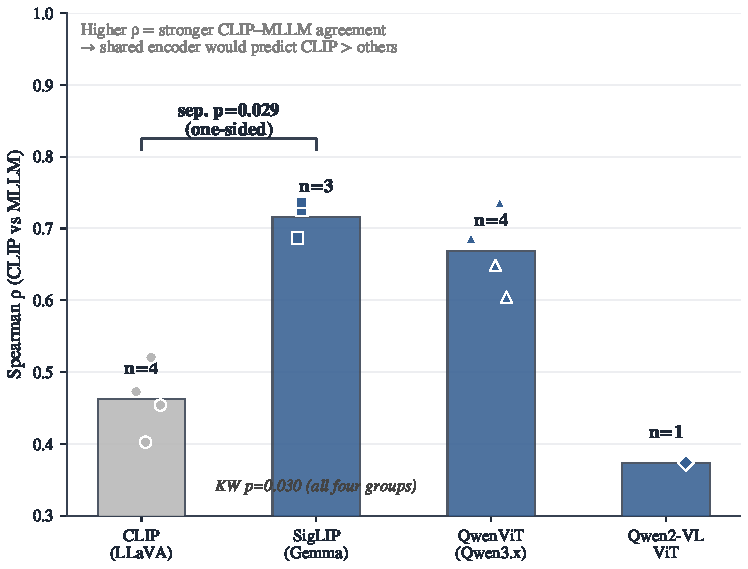
\includegraphics[width=\columnwidth]{fig2_not_shared_encoder.pdf}
\caption{Group-level Spearman correlation between CLIP AnchorScore and MLLM per-class accuracy, by vision-encoder family. MLLMs with encoders different from CLIP (SigLIP $\rho=0.716$, QwenViT $\rho=0.669$) correlate more strongly than the CLIP-encoder group ($\rho=0.462$); individual model values shown as group-specific markers (full list in Supplement \S4). $n=4,3,4,1$ models per group; the hatched bar marks the $n=1$ group; SCB5, 13 pooled classes; y-axis truncated at 0.3 to emphasize ordering.}
\label{fig:ruleout}
\end{figure}

The SigLIP group, which uses a completely different vision encoder (SigLIP ViT-SO400M, trained with a pairwise ranking loss rather than CLIP's contrastive loss), shows the strongest correlation ($\rho=0.716$). The QwenViT group, using Qwen's custom encoder, is also higher ($\rho=0.669$).

 To address the concern that the original comparison rested on a single CLIP-encoder MLLM, we evaluated three additional MLLMs that share CLIP's vision encoder, LLaVA-1.5-13B, LLaVA-NeXT-Mistral-7B, and LLaVA-NeXT-Vicuna-7B, using the same evaluation protocol (class-name prompt, 100 images per class, fixed seed; \S\ref{sec:reproducibility}). Their per-class accuracies correlate with AnchorScore at $\rho=0.454$, $\rho=0.521$, and $\rho=0.402$, respectively, yielding a CLIP-group mean of $\rho=0.462$ ($n=4$). All four CLIP-encoder MLLMs fall below every SigLIP model ($\rho=0.687$--$0.736$); the seven model-level $\rho$ values separate completely by encoder family, an event with one-sided exact probability $1/\binom{7}{4}=0.029$ under the null of no group ordering.

 A Kruskal--Wallis test across all four encoder groups (CLIP, SigLIP, QwenViT, Qwen2-VL ViT; $n=4,3,4,1$ model-level $\rho$ values, respectively) gives $H=8.93$, $p=0.030$. A permutation test comparing CLIP directly against the QwenViT group (whose encoders share no architecture with CLIP) yields $p=0.029$ (permutation, $10^5$ draws), the smallest attainable two-sided value for a complete separation of $n=4$ vs $n=4$ model-level correlations: $2/\binom{8}{4}=0.029$, i.e., all $4\times 4=16$ cross-group pairwise orderings separate the two groups completely. The Qwen2-VL ViT group is a single model ($n=1$), so it participates in the omnibus test but carries no within-group variance; it does not drive the CLIP-vs-QwenViT contrast, which excludes it. Across every grouping, the CLIP group ranks lowest, and the separation is now statistically significant rather than borderline. This pattern provides evidence against Hypothesis~1: models with different encoders correlate with CLIP at least as well as the CLIP-encoder models, inconsistent with the shared-encoder account. The CLIP group still contains the lowest-accuracy MLLM in our set (LLaVA-1.5-7B, 32.5\% mean accuracy vs.\ 58.3\% for the Gemma series), but the expansion to four models across two LLaVA generations addresses the $n=1$ limitation. To test whether the low CLIP-group $\rho$ is driven by the shared LLaVA-family language decoders (Vicuna/Mistral) rather than the CLIP encoder itself, we additionally evaluated three CLIP-encoder MLLMs with non-LLaVA decoders under the same protocol: BLIP-2 OPT-2.7B (CLIP ViT-G/14 + OPT-2.7B), InstructBLIP-Flan-T5-XL (CLIP ViT-G/14 + FLAN-T5-XL), and IDEFICS-9B (OpenCLIP ViT-L/14-336 + LLaMA-1 via perceiver fusion). Their per-class correlations are $\rho=0.392$, $\rho=0.243$, and $\rho=0.168$, respectively, all at or below the CLIP-group range, spanning three decoder families (OPT, FLAN-T5, LLaMA-1) and two fusion paradigms (Q-Former and perceiver), so the low CLIP-group $\rho$ is not obviously driven solely by the shared LLaVA-family decoders. Each control nonetheless exhibits a strong class prior (near-deterministic single-attractor outputs within each sub-dataset, e.g., 78--100\% of responses map to a single class name), which limits the weight these controls can carry.

\paragraph{Within- and Between-Family Difficulty Structure.}
The decoder controls hold the encoder fixed and vary the decoder; the converse comparison asks how much of the variation in class-difficulty rankings is associated with model family at all. Using the existing per-class accuracy vectors, we computed pairwise Spearman agreement between all model pairs and partitioned them into within-family and between-family comparisons. On SCB5 (12 MLLMs, four families), within-family agreement ($0.822$, 15 pairs) substantially exceeds between-family agreement ($0.393$, 51 pairs; difference $+0.429$, exact permutation $p=0.0002$ over all 138{,}600 family-label assignments; bootstrap 95\% CI $[0.16, 0.71]$ over classes). The same direction holds on Stanford40 ($0.772$ vs.\ $0.609$; difference $+0.163$; bootstrap 95\% CI $[0.02, 0.35]$), although with six models the exact test's resolution is limited (smallest attainable $p = 1/15 \approx 0.067$), so it is read as directional rather than significant. Two features of this pattern matter. First, between-family agreement remains substantial and positive (94\% of the 51 cross-family pairs positive), consistent with a sizable cross-family shared component. Under a single-shared-factor-plus-noise model, between-family agreement reflects the product of the two models' correlations with the shared signal; the mean cross-family product of the observed per-model AnchorScore correlations ($0.337$ over the same 51 pairs) is close to the observed $0.393$ (a rough consistency check, not a fitted model). Second, the elevated within-family agreement cannot be attributed to the shared visual encoder alone. Under the same single-factor model, two models in a family would agree with each other roughly in proportion to the product of their agreements with the shared factor, whereas within-family agreement exceeds the corresponding AnchorScore--family correlations for all three multi-model families (CLIP: $0.788$ vs.\ $0.462$; QwenViT: $0.897$ vs.\ $0.669$; SigLIP: $0.742$ vs.\ $0.716$). Consistent with this, the three non-LLaVA CLIP-encoder controls above agree with each other far less ($0.220$ mean pairwise) than the LLaVA-family models do ($0.788$), although their class-prior collapse limits the weight this comparison can carry. The within--between contrast is a ranking-agreement difference, not a variance-explained estimate. A useful conceptual decomposition is therefore $D_{mc} = S_c + F_{f(m),c} + \epsilon_{mc}$: a cross-family shared class signal $S_c$ (what AnchorScore tracks), a family-conditioned component $F$, and model-specific residual variation; the present observational design cannot localize $F$ to the encoder, projector, decoder, or instruction-tuning stage. The mechanism claim of this paper concerns $S_c$; the family component delimits its scope rather than contradicting it.

 The direct geometric evidence in \S\ref{sec:geometry}, which uses independently extracted visual features and does not depend on MLLM behavioral correlations, provides the stronger test of shared class-neighborhood geometry.

This finding provides evidence that the mechanism is not specific to CLIP, albeit at the modest sample size of available encoder families. SigLIP's high group-level $\rho=0.716$ motivates direct geometric analysis; we therefore include SigLIP in the CKA and class-geometry experiments of \S\ref{sec:geometry} (the encoder used by Gemma, extracted via open\_clip with \texttt{ViT-SO400M-14-SigLIP-384} webli weights), verifying its class geometry directly rather than inferring it from downstream accuracy.

\subsection{Shared Class-Neighborhood Geometry}
\label{sec:geometry}

Having provided evidence against the trivial explanations of what the mechanism is \emph{not}, we now test what it \emph{is}: shared class-neighborhood geometry. If all vision encoders converge to similar class-neighborhood geometry, then (a) their feature spaces should be similar, and (b) their class similarity matrices should be nearly identical.

\subsubsection{Feature Space Similarity (CKA)}

We extract visual features from 160 SCB5 images (20/class) using seven encoders (three CLIP variants, QwenViT, SigLIP, ResNet-50, and DINOv2) and compute pairwise CKA. The full $7\times7$ CKA matrix with per-cell values is reported in Supplement Fig.~1.

Within the CLIP family, CKA exceeds 0.87 (LAION L/14 vs. OpenAI L/14: 0.907; LAION L/14 vs. B/32: 0.905), confirming near-identical feature spaces. Cross-encoder CKA between CLIP variants and QwenViT ranges from 0.79 to 0.82, a high value given that QwenViT is trained alongside a language model rather than with a contrastive image-text objective. SigLIP (ViT-SO400M, the encoder inside the Gemma MLLMs whose group-level correlation drives the shared-encoder test of \S\ref{sec:ruleout}) agrees with every CLIP variant at CKA $0.86$ and with QwenViT at CKA $0.84$, the highest cross-family agreement. The two more constrained controls, ResNet-50 (ImageNet-1k only) and DINOv2 (LVD-142M), reach CKA $0.80$--$0.87$ and $0.70$--$0.82$ respectively with the Internet-scale encoders. This links the behavioral evidence (SigLIP $\rho=0.716$, the strongest non-CLIP encoder) and the geometric evidence more directly, by verifying SigLIP's feature space rather than inferring its geometry from Gemma's downstream accuracy. A caveat applies to any single-scalar similarity reading: recent work shows that similarity metrics can be inflated by network scale and advocates permutation-based null-calibration \cite{groger2026aristotelian}; our Mantel comparisons are permutation-tested and span encoders of comparable scale, which partially pre-empts this confound.

This feature-level similarity is necessary but not sufficient for shared class-neighborhood geometry. The critical test is whether class-level geometry is also preserved.

\subsubsection{Class Similarity Matrix Analysis}

We directly test this by computing class centroid cosine similarity matrices for each encoder and measuring their agreement with a \emph{Mantel test}, the Spearman rank correlation between the upper triangles of two similarity matrices, with class-label permutation used to assess significance. Because SCB5 has only 8 classes (28 class pairs), asymptotic $p$-values are unreliable; we therefore use an exact permutation test that enumerates all $8! = 40{,}320$ class relabelings. For each pair of encoders we report the observed $\rho$ and the fraction of permutations whose $\rho$ meets or exceeds it.

\begin{figure*}[t]
\centering
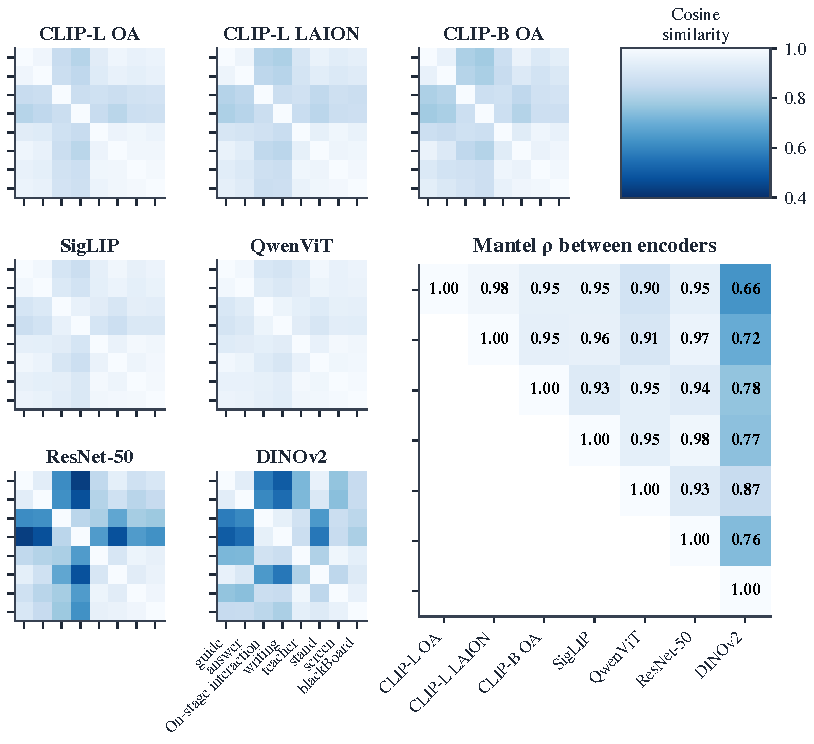
\includegraphics[width=\textwidth]{fig3_class_geometry.pdf}
\caption{Class geometry consistency across seven vision encoders. Seven $8\times8$ class-centroid similarity matrices (3 CLIP variants, QwenViT, SigLIP, ImageNet-1k-only ResNet-50, DINOv2; 50 images per class, color scale $[0.4,1.0]$) show consistent block structure despite different data, objectives, and architectures. The $7\times7$ Mantel agreement matrix (bottom right; color scale $[0.45,1.0]$, cell values annotated) reports the Spearman $\rho$ between each pair of these matrices (21 pairs, all $p<5\times10^{-5}$ by exact permutation; numerical values in \S\ref{sec:geometry}).}
\label{fig:geometry}
\end{figure*}

\Cref{fig:geometry} reveals consistent class geometry across the seven encoders. Within CLIP variants, the Mantel statistic ranges from $\rho=0.95$ to $0.98$, indicating near-identical class neighborhoods. The cross-encoder Mantel statistic between CLIP (both L/14 and B/32) and QwenViT ranges from $\rho=0.897$ to $0.949$ ($0.90$--$0.95$ after rounding). Critically, the same analysis extended to SigLIP, the encoder whose behavioral correlation ($\rho=0.716$) most strongly argues against the shared-encoder account in \S\ref{sec:ruleout}, yields Mantel $\rho=0.927$--$0.957$ against all three CLIP variants and $\rho=0.949$ against QwenViT, all with exact permutation $p<5\times10^{-5}$: no random relabeling of the 8 class labels produced agreement as high as the observed value (only the trivial identity relabeling matches). The encoder that most strongly argues against the shared-encoder account on behavioral grounds therefore shares the same class-neighborhood geometry as every other encoder, closing the gap between the behavioral and geometric evidence.

A skeptic might argue that 8 coarse classroom classes are so different from one another that any encoder would recover the same pairwise ordering, making high Mantel agreement a foregone conclusion. Four observations argue against triviality.

First, the pairwise ordering is not degenerate: the matrices contain a structured pattern of near and far pairs (e.g., \texttt{blackboard-writing} vs.\ \texttt{blackBoard}, \texttt{guide} vs.\ \texttt{stand}), and the exact permutation test shows that random relabelings of these 8 classes essentially never reproduce the observed agreement ($p<5\times10^{-5}$, the minimum attainable).

Second, the measure has discriminative resolution: agreement is systematically ordered by family (within-CLIP $0.95$--$0.98$ $>$ SigLIP-cross $0.93$--$0.96$ $>$ QwenViT-cross $0.90$--$0.95$), and this ordering, not a saturated ceiling, replicates on 40 classes (Stanford40, $\rho=0.81$ on 780 pairs) and 102 fine-grained classes (Flowers102, $\rho=0.51$--$0.83$ across ten encoder pairs), where the pairwise structure is far too dense to be recovered trivially.

Third, if the agreement merely reflected coarse semantic commonality recovered by any reasonable encoder, then the amount of training data would not matter---yet DINOv2, trained on $110\times$ more data than ResNet-50 (142M vs.\ 1.28M images) with partial overlap of CLIP's corpora, shows \emph{weaker} agreement than ResNet-50 ($\rho=0.66$--$0.87$ vs.\ $0.93$--$0.98$). The magnitude of the Mantel statistic is thus informative, not saturated: it tracks how well each encoder's training regime preserves the same class neighborhood, which is precisely the quantity this account predicts should be shared. Fourth, we confront the trivial-competence alternative directly, using the permutation null as a competence control. Two encoders that merely solve the same eight-class task, without shared fine-grained geometry, could still agree substantially because all classes carry within-domain similarity; random class relabelings of one matrix against the other therefore attain up to $|\rho|=0.944$ across the 21 pairs (10{,}000 relabelings per pair, seed 42; \texttt{analysis/mantel\_null\_baseline.py}). Yet every observed agreement exceeds the maximum permuted agreement for its pair (margins $+0.01$ to $+0.12$), and the exact enumeration certifies $p<5\times10^{-5}$ throughout: the specific class-to-class pairing is not explained by shared competence alone. The raw 8-class magnitudes should nonetheless be read against this elevated baseline; the 40- and 102-class replications, where the null is far tighter, carry the informativeness claim.

All five encoders above were trained on Internet-scale corpora that partially overlap, leaving open the alternative that the shared geometry is an artifact of training-data overlap (the H2 confound of \S\ref{sec:intro}). We test this directly by adding a sixth encoder with a sharply constrained, well-characterized training set: a supervised \textbf{ResNet-50 trained on ImageNet-1k only} \cite{he2016deep} (1.28M images, 1000 classes, the full training set is public). ResNet-50's SCB5 class geometry agrees with every other encoder at Mantel $\rho=0.928$--$0.980$ (vs.\ CLIP-L LAION $0.967$, CLIP-L OpenAI $0.950$, CLIP-B/32 $0.936$, QwenViT $0.928$, SigLIP $0.980$; all exact-permutation $p<5\times10^{-5}$), vying with the within-CLIP pair (CLIP-L OpenAI vs.\ CLIP-L LAION, $\rho=0.981$) for the highest agreement in the entire panel. A supervised ImageNet-1k-only encoder therefore recovers the same class-neighborhood structure as Internet-scale contrastive and language-model-pretrained encoders, which is difficult to attribute to data overlap and instead supports the natural-image-distribution interpretation.

We also add a \textbf{DINOv2 ViT-B/14} \cite{oquab2024dinov2} (self-supervised on LVD-142M, which partially overlaps LAION) as an intermediate case: it agrees more modestly ($\rho=0.66$--$0.87$). The fact that DINOv2, trained on far \emph{more} data than ResNet-50 and with \emph{more} overlap with CLIP's corpora, shows \emph{weaker} geometric agreement than ResNet-50 is the opposite of what a simple monotonic data-overlap account would predict, and further weakens H2. The lower agreement also shows that convergence is not monotone in data scale alone: the interaction between training objective and data distribution matters, but our experiments do not adjudicate between a supervised-objective account (supervised ResNet-50 anchored to human category structure) and a self-supervised account (DINOv2 free to organize inter-class distances without language supervision). This remains an unresolved boundary condition rather than a settled mechanism.

This provides direct evidence for shared class-neighborhood geometry: when two classes are close in one encoder's space, they are also close in another encoder's space. Across the seven encoders studied here (three CLIP variants, SigLIP, QwenViT, ResNet-50, DINOv2), these results are consistent with broadly shared class geometry; the training-data-overlap account (H2) is addressed directly by the ResNet-50 result above and is substantially weakened, though not fully excluded, as a standalone explanation (see \S\ref{sec:discussion}).

\subsubsection{Class-Prototype Geometry Versus Patch Features}
\label{sec:patchlevel}

A natural reading of the high cross-encoder CKA ($0.79$--$0.87$) and class-level Mantel $\rho$ ($0.90$--$0.96$) is that one encoder's features are directly mappable to another's, so the entire feature space is shared, not merely the class-neighborhood structure. We tested this directly. For each non-CLIP encoder $E \in \{\text{SigLIP}, \text{CLIP-B/32}, \text{QwenViT}\}$ we trained a label-free two-layer MLP ($d_E \to 2048 \to 1024$, GELU, dropout $0.1$, 12 epochs, AdamW) to map $E$'s \emph{per-patch} features into CLIP ViT-L/14's per-patch feature space on 4{,}896 SCB5 training images, and evaluated $R^2$ on 500 held-out validation images. To rule out leakage we audited the data splits. Within any single SCB dataset, the train and val directories share no filenames (0 overlap in all three datasets), so the per-dataset, zero-shot accuracy evaluations behind the core correlations are unaffected. Across datasets, however, the same byte-identical image sometimes appears in one dataset's train split and another's val split (cross-dataset duplication, verified by md5). In the pooled 5,000-image training pool we use here, 104 such images collided by filename with pooled val images, so we removed them from the training set before fitting the adapter; the 500 validation images contain none of the leaked filenames (confirmed empirically), so the reported $R^2$ is on a fully train-disjoint sample.

\Cref{tab:patchlevel} contrasts per-patch mapping $R^2$ against the class-centroid Mantel RSA on the same encoder pairs. A linear ridge adapter recovers at most $R^2 = 0.19$ ($0.05$--$0.19$ across encoders) of per-patch variance; the two-layer MLP does not improve on it ($R^2 = 0.036$--$0.209$ on the independent validation set, better than the linear adapter only for SigLIP), while a pure-noise control is negative as expected. The class-centroid similarity matrices of the same encoder pairs, by contrast, agree at Mantel $\rho = 0.90$--$0.96$. The $4$--$5\times$ gap is consistent with this interpretation: encoders diverge substantially in their per-patch representations, with at most $21\%$ of patch-feature variance transferable across families, yet converge tightly on the pairwise similarity structure of class \emph{prototypes} (centroids). The shared geometry is therefore strongest at the class-prototype level rather than in raw per-patch feature spaces, emerging clearly only after averaging over patches and images. This localizes the strongest observed structural correspondence to the class-prototype level: the natural-image distribution constrains which \emph{classes} look similar (a statistical regularity over class centroids), without forcing encoders to agree on how individual image patches are encoded, consistent with the broadly shared visual structure interpretation and the three-level distinction (geometry $\to$ confusability $\to$ difficulty) of \S\ref{sec:intro}.

\begin{table}[h]
\centering
\caption{Per-patch feature transferability versus class-prototype geometry across encoder pairs. Shared geometry is strongest at the class-prototype level rather than the patch-feature level.}
\label{tab:patchlevel}
\small
\begin{tabular}{lccc}
\toprule
Encoder (vs.\ CLIP ViT-L/14) & Linear $R^2$ & MLP $R^2$ & Class Mantel RSA \\
\midrule
SigLIP ViT-SO400M & 0.192 & 0.209 & 0.93--0.96 \\
CLIP ViT-B/32 & 0.135 & 0.129 & 0.95 \\
QwenViT & 0.053 & 0.036 & 0.90--0.95 \\
\midrule
Gaussian noise (null control) & $-0.000$ & $-0.120$ & --- \\
\bottomrule
\end{tabular}

\vspace{2pt}
{\footnotesize $R^2$: variance of CLIP ViT-L/14 patch features explained by an adapter (linear ridge, or 2-layer MLP with 2048 and 1024 hidden units, 12 epochs) trained on 4{,}896 non-leaked SCB5 train images, evaluated on 500 fully-disjoint validation images. Class Mantel RSA: Spearman $\rho$ between $8\times8$ class-centroid cosine-similarity matrices on SCB5 (\S\ref{sec:geometry}).}
\end{table}

\subsection{Mediation Through Shared Per-Class Difficulty}
\label{sec:mediation}

If shared class-neighborhood geometry underlies the AnchorScore--MLLM relationship, then a measure of shared per-class difficulty should account for a large part of the association. We test this via a nonparametric bootstrap mediation analysis (product-of-coefficients on standardized ranks, 10{,}000 class resamples; see \S\ref{sec:reproducibility}). For each MLLM, the predictor $X$ is AnchorScore; the mediator $M$ is the leave-one-out cross-model average per-class accuracy (excluding the target model to avoid circularity); and the outcome $Y$ is the target MLLM's per-class accuracy. The mediation uses the nine core MLLMs whose full per-class accuracy vectors are persisted from the benchmark; the three LLaVA models added in \S\ref{sec:ruleout} for the shared-encoder test were evaluated at 100 images per class under a separate protocol and are excluded here to keep the predictor, mediator, and outcome on a common per-class scale. We report indirect effects $a\times b$ (the product of the AnchorScore$\rightarrow$mediator and mediator$\rightarrow$MLLM paths), direct effects $c'$ (the residual AnchorScore$\rightarrow$MLLM association after controlling for the mediator), and bootstrap 95\% confidence intervals for both.

\Cref{tab:mediation} shows the results. On SCB5 ($n=13$ pooled classes), eight of nine indirect-effect point estimates are positive and consistent with mediation; the sole exception is LLaVA-1.5-7B, for which $a\times b=-0.16$ with $c'=0.64 > c=0.47$. This sign pattern is the classic \emph{suppression} configuration: the leave-one-out cross-model difficulty score is positively associated with AnchorScore ($a=0.76$) but negatively with LLaVA-1.5-7B's accuracy once AnchorScore is controlled ($b=-0.22$), so the indirect path runs counter to the total association. This is consistent with LLaVA-1.5-7B being an outlier among our MLLMs: it has the lowest mean accuracy in our set (32.5\%) and shows anomalously low agreement with other MLLMs ($\rho=0.03$ to $0.37$ across all eight other models, \S\ref{sec:phenomenon}), and suggests its difficulty profile does not follow the cross-model consensus that mediates the correlation for the other models. Bootstrap confidence intervals are very wide, a direct consequence of the small class count; the intervals for all nine SCB5 models span zero (Table~\ref{tab:mediation}). The large intervals do \emph{not} constitute evidence of zero residual effect; rather, the analysis lacks sufficient statistical power with only 13 classes.

 On Stanford40 ($n=40$), where power is substantially higher, the indirect effects are consistently significant (all six models' 95\% bootstrap CIs exclude zero), with point estimates ranging from $0.449$ to $0.714$. The residual direct effects are small: $c' = -0.134$ to $+0.229$, with all six CIs containing zero. One interpretive caveat applies: 37 of the 40 Stanford40 classes have AnchorScore above 60\%, so the difficulty ranking that drives the mediation is concentrated in a few low-AnchorScore classes rather than spread across the full difficulty spectrum; the Stanford40 mediation therefore demonstrates the shared-difficulty pathway where AnchorScore has discriminative leverage, and should not be read as evidence of fine-grained per-class mediation. SCB5 provides directional consistency (eight of nine models have positive indirect-effect point estimates, sign test $p=0.020$) but all nine CIs span zero, reflecting the limited statistical power at $n=13$; the Stanford40 analysis provides the powered test. Collinearity diagnostics (VIFs in Table~\ref{tab:mediation}) and counterfactual mediator controls (Supplement \S3) rule out severe collinearity artifacts and confirm that the mediation is specific to the genuine shared-difficulty signal rather than to the pipeline itself.

Overall, these results are consistent with substantial mediation of the AnchorScore--MLLM relationship by shared per-class difficulty on Stanford40, with SCB5 providing directional support at lower power. A mediation analysis is an association-based decomposition, not a causal proof: it quantifies how much of the correlation flows through the mediator, but a significant indirect effect does not by itself demonstrate that shared difficulty \emph{causes} the MLLM correlation. The mediator is by construction the cross-model shared signal, so the mediation's role here is the quantification of the shared-difficulty component; the structural account of its origin is supplied by the geometric evidence of \S\ref{sec:geometry}, not by the mediation itself. The geometric evidence in \S\ref{sec:geometry} provides independent support for the interpretation that this shared difficulty reflects underlying shared class geometry; however, the geometry$\rightarrow$difficulty link is correlational and alternative mechanisms remain unadjudicated (see \S\ref{sec:discussion}). Two such alternatives and three further checks of the mediation analysis itself follow.

\textbf{Assessing the shared-image-difficulty alternative.}
A potential concern is that the mediator (leave-one-out cross-model per-class accuracy) could in principle capture \emph{image-level} difficulty, where some classes simply contain intrinsically harder images, rather than \emph{class-neighborhood geometry} per se; under that account the AnchorScore--MLLM correlation would not require geometric convergence at all. Three pieces of internal evidence substantially constrain this alternative, though they do not eliminate it.

 First, if raw image difficulty alone drove the correlation, all three CLIP variants evaluated on the \emph{same} images would predict MLLM difficulty equally well; instead, AnchorScore computed with CLIP ViT-L/14 (LAION-2B) reaches $\rho=0.73$ (vs.\ Gemma4-31B), while the OpenAI-trained ViT-L/14 reaches only $\rho=0.58$ and ViT-B/32 only $\rho=0.39$ (\S\ref{sec:sensitivity}). Because the three variants are scored on the identical image set, image difficulty is held constant; the $\approx 2\times$ spread in predictive power therefore reflects model-specific differences in visual representation and/or text--image alignment rather than image difficulty alone, consistent with an encoder-side (though not exclusively geometric) account (and with ViT-B/32's known noisier zero-shot estimates, whose underlying class geometry is nonetheless preserved: Mantel $\rho=0.949$ with QwenViT). This shows that image difficulty alone cannot explain the full pattern, but does not exclude a contributing role. Second, the cross-encoder Mantel agreement ($\rho\approx0.81$--$0.95$) is measured directly on class-centroid similarity matrices, not on per-image accuracies, so it cannot be inflated by shared image difficulty.

 Third, the prompt-variant experiment (\S\ref{sec:prompt}) shows that CLIP's most striking failures are resolved without any change to the \emph{image}, purely by changing the text alignment, showing that useful visual information was available on the very classes where accuracy was lowest. These analyses substantially constrain the image-difficulty alternative, but do not exclude the possibility that class-level image difficulty contributes to the observed correlation alongside shared geometry. The geometric evidence provides an independently observable structural correlate of cross-model difficulty; whether it is the dominant cause awaits perturbation-based validation (see Limitations).

\textbf{Counterfactual mediation controls.}
A second potential concern is that the mediator itself is \emph{internal to the MLLM system}: AnchorScore and the leave-one-out cross-model mean accuracy are measured on the same images, so the indirect effect could in principle be an artifact of the mediation pipeline rather than of shared difficulty. We therefore reran the same cluster-bootstrap pipeline under three counterfactual mediator specifications, holding everything else fixed (seed, resampling, estimator; \texttt{analysis/mediation\_counterfactual\_controls.py}). First, a \emph{class-permuted} mediator: the leave-one-out means with class labels permuted (seed 42), which preserves their marginal distribution while destroying any true per-class signal. Second, a \emph{random-noise} mediator (fixed per-model seed), which cannot carry difficulty information at all. Third, on SCB5 only, an \emph{independent-encoder} mediator: per-class accuracy of OpenAI-trained ViT-L/14 and ViT-B/32 (the same evaluation pipeline as AnchorScore but with checkpoints outside the nine-model MLLM system and outside the LAION anchor), from the committed multi-backbone snapshot. On Stanford40, where the analysis is powered, the baseline indirect effect is significant ($+0.56$, 95\% CI $[0.37, 0.71]$, $p<0.0001$) but the permuted ($-0.006$, CI $[-0.06, 0.04]$) and noise ($-0.02$, CI $[-0.06, 0.02]$) mediators produce no indirect effect at all: the pipeline attributes nothing when the mediator's class signal is destroyed, and the significant baseline result is specific to the genuine shared-difficulty mediator. On SCB5 the baseline replicates the combined-test result of \S\ref{sec:mediation} ($+0.54$, CI $[-0.51, +0.89]$, $p=0.089$), and the permuted ($-0.04$) and noise ($-0.02$) mediators again collapse. The independent-encoder controls on SCB5 are not significant ($+0.005$ and $+0.003$), but this is a sample-size limitation rather than evidence against the mechanism: at $n=13$, these mediators have substantially weaker $a$-paths to the anchor than the LOO MLLM mean (Spearman $\rho=0.24$--$0.60$ vs.\ $0.87$), so even a true indirect effect of comparable per-class magnitude cannot be resolved; Stanford40, which is powered, cannot run this control because no multi-backbone anchors exist for it. Full numbers in Supplement \S3.

\begin{table}[h]
\centering
\caption{Bootstrap mediation: $c$ total, $c'$ direct, $a\times b$ indirect effect through shared difficulty. Bold: 95\% CI excludes zero; $\dagger$: suppression (see note).}
\label{tab:mediation}
\small
\begin{tabular}{lcccccl}
\toprule
\multirow{2}{*}{Model} & \multirow{2}{*}{$c$} & \multirow{2}{*}{$c'$} & \multicolumn{2}{c}{$a\times b$} & \multirow{2}{*}{Prop.} & \multirow{2}{*}{VIF} \\
\cmidrule{4-5}
& & & indirect & 95\% CI & & \\
\midrule
\multicolumn{7}{c}{\textit{SCB5 (n=13), low power (CIs span zero)}} \\
\midrule
LLaVA-1.5-7B & 0.47 & 0.64 & $-$0.16 & [$-$1.41, 0.28] & $-$0.35$^{\dagger}$ & 2.4 \\
Qwen3.5-27B  & 0.60 & 0.06 & 0.55 & [$-$0.86, 1.10] & 0.91 & 2.6 \\
Qwen3.6-27B  & 0.65 & $-$0.01 & 0.66 & [$-$0.88, 1.02] & 1.02$^{\dagger}$ & 2.7 \\
Qwen3.5-35B-A3B  & 0.74 & 0.12 & 0.61 & [$-$0.08, 1.21] & 0.83 & 2.7 \\
Qwen3.6-35B-A3B  & 0.69 & $-$0.03 & 0.71 & [$-$0.64, 1.10] & 1.04$^{\dagger}$ & 2.7 \\
Gemma-3-27B  & 0.69 & 0.25 & 0.43 & [$-$1.07, 1.21] & 0.63 & 3.0 \\
Gemma4-31B   & 0.73 & 0.28 & 0.44 & [$-$1.08, 0.97] & 0.61 & 2.6 \\
Gemma4-26B-A4B   & 0.74 & 0.04 & 0.70 & [$-$0.25, 1.26] & 0.95 & 2.7 \\
Qwen2-VL-7B  & 0.37 & $-$0.51 & 0.88 & [$-$1.57, 1.71] & 2.37$^{\dagger}$ & 4.2 \\
\midrule
\multicolumn{7}{c}{\textit{Stanford40 (n=40)}} \\
\midrule
Qwen3.5-27B       & 0.58 & $-$0.13 & \textbf{0.71} & [0.37, 0.94] & 1.23$^{\dagger}$ & 3.0 \\
Qwen3.5-35B-A3B   & 0.64 & 0.04 & \textbf{0.60} & [0.26, 1.02] & 0.94 & 3.1 \\
Qwen3.6-27B       & 0.72 & 0.23 & \textbf{0.50} & [0.17, 0.97] & 0.69 & 2.5 \\
Qwen3.6-35B-A3B   & 0.72 & 0.22 & \textbf{0.51} & [0.16, 0.85] & 0.70 & 2.9 \\
Gemma4-26B-A4B    & 0.68 & 0.23 & \textbf{0.45} & [0.06, 0.72] & 0.66 & 2.7 \\
Gemma4-31B        & 0.66 & 0.06 & \textbf{0.61} & [0.23, 0.96] & 0.92 & 2.9 \\
\bottomrule
\end{tabular}

\vspace{2pt}
{\footnotesize 10{,}000 class resamples, product-of-coefficients on standardized ranks. $c$: total AnchorScore--MLLM correlation (Spearman $\rho$); $c'$: direct effect after controlling for the leave-one-out cross-model average difficulty; $a\times b$: indirect effect through shared difficulty. Bootstrap 95\% CIs (percentile) in square brackets; SCB5 CIs span zero for all nine models, reflecting low power. VIF: variance inflation factor between AnchorScore and mediator. $\dagger$: proportion mediated $(c-c')/c$ outside $[0,1]$ (suppression); the indirect path accounts for at least the full total association and should not be read as a literal fraction.}
\end{table}

\textbf{Mediation sensitivity analysis.}
To quantify how robust the Stanford40 indirect effect is to unmeasured mediator--outcome confounding, the sensitivity analysis of Imai, Keele and Yamamoto is applied \cite{imai2010sensitivity} (Theorem 4 closed form; cluster-bootstrap percentile CI over the same 10{,}000 class resamples). The sensitivity parameter $\rho = \mathrm{Corr}(\varepsilon_M, \varepsilon_Y \mid X)$ measures the residual correlation between the mediator and outcome models that would have to exist under violation of sequential ignorability (i.e., an unmeasured pre-treatment confounder of the $M\rightarrow Y$ path). At $\rho=0$ (the paper's baseline assumption) the parametric indirect effect is $+0.562$, 95\% CI $[0.371, 0.708]$, matching the product-of-coefficients estimate. The CI first includes zero at $|\rho|=0.35$ ($R^2_M \cdot R^2_Y$ equivalent $\approx 0.12$), meaning an unmeasured confounder would have to explain roughly 12\% of the residual variance in both the mediator and outcome models to overturn the indirect effect. This is a non-trivial threshold: a candidate confounder such as shared image difficulty would need to operate at this magnitude, and the counterfactual controls above (permuted and noise mediators collapse to zero) indicate the pipeline does not fabricate indirect effects at smaller confounder strengths. SCB5 ($n=13$) lacks power for sensitivity estimation, as its baseline CI already spans zero. We report this as a parametric linear structural equation model (LSEM) robustness check complementary to the nonparametric cluster-bootstrap rank-z mediation used throughout the paper.

\textbf{Power analysis.}
An explicit power analysis supplements the confidence intervals (Fisher-$z$ asymptotic approximation). At the SCB5 sample size ($n=13$), power to detect a residual direct effect of $|\rho|=0.30$ is only 16\%, and even $|\rho|=0.45$ reaches 33\% power. A two-sided test on 13 classes achieves 80\% power only for $|\rho|\geq0.71$. At $n=40$ (Stanford40), power reaches 80\% at $|\rho|\geq0.43$, and the observed $c'$ values ($-0.13$ to $0.23$) fall below this threshold. These figures quantify this concern: the wide confidence intervals and nonsignificant partial associations primarily reflect limited statistical power rather than definitive evidence of zero residual effect. On Stanford40, however, the consistently significant indirect effects and small direct-effect point estimates remain informative.

\textbf{Combined test across models.}
Although no single SCB5 model's indirect-effect CI excludes zero, the \emph{cross-model agreement} carries independent evidence. Eight of the nine SCB5 models have positive indirect-effect point estimates (the sole exception being the outlier LLaVA-1.5-7B, \S\ref{sec:mediation}); a binomial sign test rejects a zero-median null at $p=0.020$ (one-sided). Treating the nine indirect-effect point estimates as exchangeable replicates, a Wilcoxon signed-rank test gives $p=0.004$ and a one-sample $t$-test gives $p<0.001$ (both one-sided), though these anti-conservative tests assume between-model independence that the shared classes violate. The most conservative combination, a cluster bootstrap that resamples the 13 classes (cluster unit) and, within each resample, averages the indirect effect across the nine models, yields a pooled mean indirect effect of $+0.54$ with 95\% CI $[-0.51, +0.89]$ ($p=0.089$, one-sided), which respects the class-level clustering but still straddles zero. Thus the direction of the SCB5 indirect effect is consistently positive across models (sign test significant), while its magnitude, as expected at $n=13$, is poorly resolved by the class-clustered bootstrap; the Stanford40 analysis ($n=40$, all six indirect CIs excluding zero) provides the higher-powered confirmation (\texttt{analysis/mediation\_combined\_test.py}).

\subsection{Semantic Versus Visual Origins of CLIP Failures}
\label{sec:prompt}

As a convergent test, the shared-geometry account (H3) is distinguished from the raw-image-difficulty alternative (H4): perhaps the CLIP--MLLM correlation reflects intrinsic image-level hardness rather than anything encoder-specific. The two accounts make opposite predictions about reparability. Under H4, hard images are hard independent of labeling, so changing only the text side of the image--text alignment should not rescue CLIP's failures. Under H3, CLIP's failures on hard classes are expected to stem from encoder-side text--image misalignment with the visual features themselves intact, so a more descriptive prompt should repair accuracy without touching the images. We engineer prompt variants for divergent classes, the classes where CLIP has low accuracy, replacing bare class names with descriptive phrases. The five classes tested (\texttt{blackboard-writing}, \texttt{answer}, \texttt{blackBoard}, \texttt{stand}, \texttt{screen}) are the five lowest-accuracy TeacherBehavior classes under the OpenAI ViT-L/14 multi-backbone evaluation, with bare-class zero-shot accuracies in the prompt experiment of $45.3\%$, $0.0\%$, $1.7\%$, $0.0\%$, and $0.0\%$ respectively. Under the LAION-2B ViT-L/14 AnchorScore weights used throughout this paper, the same five classes score $26.1\%$, $5.6\%$, $3.2\%$, $9.6\%$, and $40.5\%$ (\S\ref{sec:setup}); four of them are the four lowest-accuracy classes under that variant, while \texttt{screen} sits mid-pack (above \texttt{guide} at $29.3\%$, below \texttt{teacher} at $50.5\%$), so the intervention covers every class at the low-accuracy end of the evaluation used, without omitting any low-accuracy class from consideration on the basis of later outcomes.

\begin{figure}[htbp]
\centering
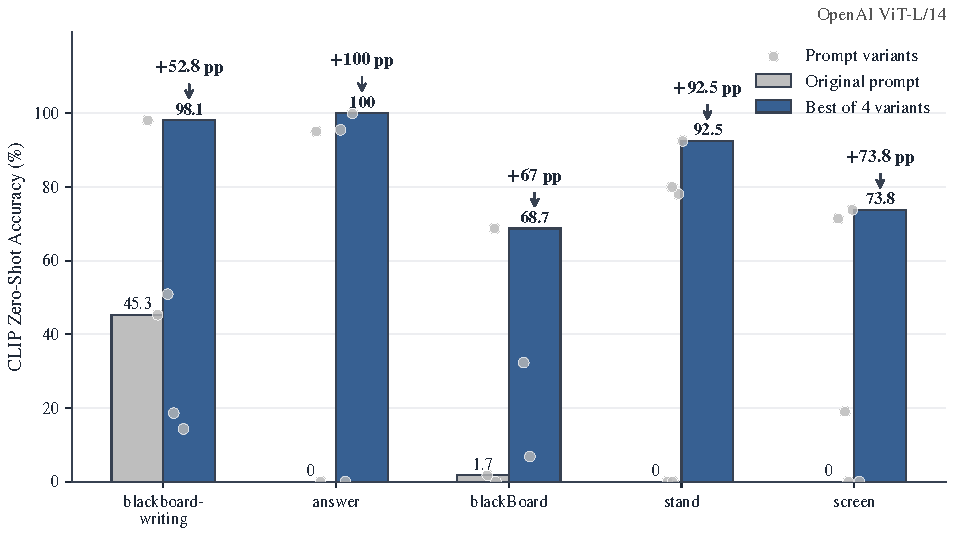
\includegraphics[width=\columnwidth]{fig4_prompt_variants.pdf}
\caption{Prompt variants resolve CLIP failures on composition classes: replacing the class name with a descriptive phrase dramatically improves accuracy on all five low-accuracy classes. OpenAI ViT-L/14; $n=42$--$439$ validation images per class; bars show the bare class-name prompt vs.\ the best of four descriptive variants (all variants shown as points); the y-axis extends past 100\% as a tick-free annotation zone for the gain labels (ticks stop at 100\%); for example, ``answer'' rises from 0\% to 100\% with ``a student raising hand to answer''.}
\label{fig:prompt}
\end{figure}

All five divergent classes show dramatic improvement (\Cref{fig:prompt}): \texttt{blackboard-writing} rises from 45\% to 98\%, \texttt{answer} from 0\% to 100\%, \texttt{blackBoard} from 2\% to 69\%, \texttt{stand} from 0\% to 92.5\%, and \texttt{screen} from 0\% to 73.8\%. Not every variant helps (for \texttt{blackboard-writing}, ``a blackboard with writing on it'' scores 14\%, below the bare class name), so the result is reparability by an appropriate description rather than robustness to arbitrary rephrasing; \Cref{fig:prompt} shows all tested variants per class. The most striking case is ``answer'': 0\% accuracy with the bare class name, but 100\% with ``a student raising hand to answer.'' This supports the interpretation that CLIP's vision encoder can perceive these concepts; its failures lie in text-image alignment rather than in the class-neighborhood geometry, consistent with text-based decompositions of CLIP's representation space \cite{gandelsman2023interpreting}. Useful visual information was thus available to the encoder on these classes, but the mapping from visual features to class labels was misaligned under the original class-name prompt. This substantially constrains H4: the difficulty signal cannot be exclusively raw image hardness, since changing only the text side of the alignment rescues accuracy on the same images; the failures involve encoder-side text--image misalignment rather than intrinsically hard images alone. However, it does not exclude the possibility that image difficulty contributes to other classes' shared difficulty patterns.

\subsection{Independent Replication on Stanford40}
\label{sec:stanford40}

The Stanford40 replication provides additional evidence across 40 independent classes. \Cref{fig:stanford40}a shows the per-class scatter ($\rho=0.817$, $p<0.001$), replicating the CLIP--MLLM relationship on an independent domain. The correlation is not driven by a few low-anchor classes: removing the three lowest-AnchorScore classes leaves $\rho=0.768$ and removing the five lowest leaves $\rho=0.738$ (both $p<0.001$), and a jackknife over the 40 classes changes $\rho$ by at most $0.043$ (\texttt{analysis/prevalence\_and\_leverage\_controls.py}).

To test whether this reflects shared \emph{feature} geometry rather than shared behavioral difficulty, we compute real 40$\times$40 class-similarity matrices directly from encoder features on all 9{,}532 Stanford40 images: for each of CLIP ViT-L/14 and the Qwen2-VL vision encoder (QwenViT, an independently trained architecture from a different family), we extract per-image features, build L2-normalized per-class centroids, and take their cosine similarities. \Cref{fig:stanford40}b compares the two matrices via a Mantel test across all 780 class pairs: the agreement is strong ($\rho=0.810$, permutation $p<10^{-4}$), indicating that two encoders with disjoint architectures and training objectives converge to largely the same class-prototype neighborhood structure. \Cref{fig:stanford40}c,d display the two matrices under a shared hierarchical-clustering order: the block structure, groups of visually similar actions, is visually preserved across encoders. This provides further support for the interpretation that the Stanford40 replication reflects shared feature geometry rather than an artifact of accuracy profiles, extending the mechanism to a natural action benchmark.

\begin{figure*}[t]
\centering
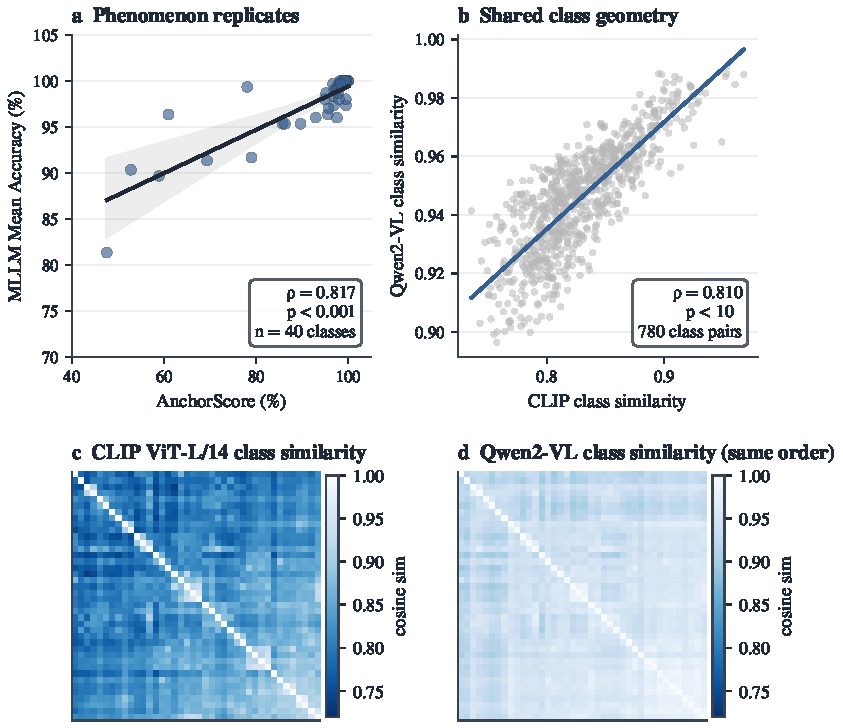
\includegraphics[width=\textwidth]{fig5_stanford40.pdf}
\caption{Stanford40 cross-dataset validation from real features (40 classes, 9{,}532 images). \textbf{(a)} Per-class AnchorScore vs.\ mean MLLM accuracy over six Ollama MLLMs; the dark line is the OLS fit and the shaded band its 95\% bootstrap band (2{,}000 resamples). \textbf{(b)} Entry-wise agreement between the CLIP and QwenViT class-similarity matrices (780 class pairs; line: OLS fit). \textbf{(c),(d)} The two $40\times40$ class-centroid similarity matrices under a shared hierarchical-clustering order.}
\label{fig:stanford40}
\end{figure*}

\subsection{Cross-Domain Validation on Flowers102}
\label{sec:flowers102}

\Cref{tab:flowers102} reports a second independent validation of the geometric convergence on \textbf{Flowers102} \cite{nilsback2008flowers}, a fine-grained benchmark of 102 flower species whose confusability structure is entirely unrelated to the classroom and action domains. We extract features from 2{,}040 images (20 per class, the same per-class budget as the SCB5 CKA analysis of \S\ref{sec:geometry}) with five encoders, the three CLIP variants, SigLIP, and QwenViT, using each encoder's canonical preprocessing, and compute 102$\times$102 class-centroid cosine-similarity matrices (5{,}151 class pairs, versus 28 on SCB5 and 780 on Stanford40). Because exact enumeration is intractable at 102 classes, significance is assessed with 10{,}000 random class-label permutations (seed 42).

\begin{table}[h]
\centering
\caption{Mantel test on Flowers102: pairwise agreement of class-centroid geometry across five encoders.}
\label{tab:flowers102}
\small
\begin{tabular}{llcc}
\toprule
Encoder pair & Family relation & $\rho$ & $p$ \\
\midrule
CLIP-L/14 (OA) vs.\ CLIP-L/14 (LAION) & within-CLIP & 0.802 & $<0.0001$ \\
CLIP-L/14 (OA) vs.\ CLIP-B/32 (OA) & within-CLIP & 0.789 & $<0.0001$ \\
CLIP-L/14 (LAION) vs.\ CLIP-B/32 (OA) & within-CLIP & 0.828 & $<0.0001$ \\
CLIP-L/14 (OA) vs.\ SigLIP & cross-family & 0.751 & $<0.0001$ \\
CLIP-L/14 (LAION) vs.\ SigLIP & cross-family & 0.683 & $<0.0001$ \\
CLIP-B/32 (OA) vs.\ SigLIP & cross-family & 0.590 & $<0.0001$ \\
CLIP-L/14 (OA) vs.\ QwenViT & cross-family & 0.574 & $<0.0001$ \\
CLIP-B/32 (OA) vs.\ QwenViT & cross-family & 0.535 & $<0.0001$ \\
CLIP-L/14 (LAION) vs.\ QwenViT & cross-family & 0.525 & $<0.0001$ \\
SigLIP vs.\ QwenViT & cross-family & 0.514 & $<0.0001$ \\
\bottomrule
\end{tabular}

\vspace{2pt}
{\footnotesize 102 fine-grained flower classes, 20 images per class. $\rho$: Spearman correlation of the upper triangles of class-centroid cosine-similarity matrices (5{,}151 class pairs). $p$: fraction of 10{,}000 random class-label permutations whose $\rho$ meets or exceeds the observed value (smallest attainable $=10^{-4}$). OA: OpenAI weights; LAION: LAION-2B open\_clip weights; QwenViT: Qwen2-VL vision encoder.}
\end{table}

All ten pairwise agreements are significant at $p<0.0001$, the smallest attainable value at 10{,}000 permutations, showing that every encoder pair shares nontrivial class-neighborhood structure on a domain whose fine-grained confusability pattern is independent of the training corpora involved. A similar ordering is observed across the three benchmarks, although the absolute agreement decreases substantially on the fine-grained Flowers102 benchmark: within-CLIP agreement is highest ($\rho=0.79$--$0.83$), cross-family agreement with SigLIP is intermediate ($\rho=0.59$--$0.75$), and QwenViT is again the most distant encoder ($\rho=0.52$--$0.57$ against the CLIP variants, $\rho=0.514$ against SigLIP), the same encoder whose MLLM (Qwen2-VL-7B) shows the lowest behavioral correlation with AnchorScore on SCB5 ($\rho=0.374$, \S\ref{sec:phenomenon}), consistent with the shared-geometry account. Absolute agreement is lower on Flowers102 than on the 8-class SCB5 panel ($\rho=0.90$--$0.98$) and the 40-class Stanford40 panel ($\rho=0.81$); this is best read as consistent with attenuation by the fine-grained nature of the benchmark (dense confusability among 102 species) and the modest 20-image-per-class centroid budget. Two observations support this reading rather than a genuine disappearance of shared structure. First, the attenuation is uniform across family relation. The within-CLIP pair (CLIP-L/14 OA vs.\ LAION) has nearly identical features (CKA $0.91$ on SCB5) and achieves the panel's highest agreement on SCB5 ($\rho=0.981$ with 50 images/class); it drops to only $\rho=0.802$ here, a decline as large as that of the cross-family pairs. If the lower agreement reflected a real reduction of shared geometry on fine-grained classes, this near-identical pair would not be expected to lose as much as pairs that genuinely differ in architecture and training data; the uniform drop is instead consistent with the estimator being attenuated by the combination of 5{,}151 pairs (dense rank comparisons), only 20 images per class (2.5$\times$ fewer than the SCB5 centroid budget), and the fine-grained structure. Second, the behavioral stage below (Tab.~\ref{tab:flowers102b}) confirms that the shared signal survives at the class level: per-class difficulty estimated from these same 20-image centroids is significantly shared for all fifteen encoder pairs under margin difficulty ($p<0.0004$), with the correlation magnitude ($\rho=0.37$--$0.88$) comparable to the geometric $\rho$ values reported here. With 5{,}151 class pairs, the permutation test also removes the small-pair-count caveat of the 28-pair SCB5 analysis.

The geometry result establishes that encoders \emph{represent} difficulty similarly; it does not by itself show that they \emph{behave} similarly. \Cref{tab:flowers102b} closes this gap with a behavioral transfer test: we train a 1-shot logistic probe on the same 2{,}040 features from each of six encoders (the five above plus a clean supervised baseline, ResNet-50, ImageNet-1k) and define per-class difficulty twice: held-out accuracy and the mean probability assigned to the true class (margin). To keep difficulty estimates comparable and reproducible across encoders, all six probes are evaluated on twenty identical train/holdout class-balanced splits (seed 42), and significance is assessed with 10{,}000 random class permutations. Margin-based difficulty, which is less prone to quantization at high accuracy, is significantly shared for \emph{all} fifteen encoder pairs ($p<0.0004$, $\rho=0.37$--$0.88$), including the clean ResNet-50 against every Internet-scale encoder ($\rho=0.38$--$0.73$) and QwenViT against CLIP ($\rho=0.37$--$0.51$). Accuracy-based difficulty agrees for fourteen of fifteen pairs ($p<0.02$); the single exception is SigLIP vs.\ ResNet-50 ($\rho=0.18$, $p=0.069$), the pair combining the highest and lowest overall accuracy, where the SigLIP difficulty vector is strongly compressed toward 100\% even at one shot. The behavioral transfer thus provides a complementary class-level difficulty correlate of the geometric convergence, across architectures (ViT, ConvNet), objectives (contrastive, language-model-coupled, supervised), and data sources (web-scale, ImageNet-1k). We treat the probe-derived difficulty as a behavioral proxy of representation quality rather than as a direct estimate of each encoder's intrinsic classification error; because all probes share identical splits, split noise is common across encoders and does not inflate the pairwise agreement.

\begin{table}[h]
\centering
\caption{Shared per-class difficulty on Flowers102: 1-shot probe, 15 encoder pairs. Acc: per-class held-out accuracy; margin: per-class mean true-class probability.}
\label{tab:flowers102b}
\small
\begin{tabular}{llcc}
\toprule
Encoder pair & Difficulty measure & $\rho$ & $p$ \\
\midrule
CLIP-L/14 (OA) vs.\ CLIP-L/14 (LAION) & acc / margin & 0.82 / 0.86 & $<0.0001$ / $<0.0001$ \\
CLIP-L/14 (OA) vs.\ CLIP-B/32 (OA) & acc / margin & 0.72 / 0.88 & $<0.0001$ / $<0.0001$ \\
CLIP-L/14 (LAION) vs.\ CLIP-B/32 (OA) & acc / margin & 0.69 / 0.80 & $<0.0001$ / $<0.0001$ \\
CLIP-L/14 (OA) vs.\ SigLIP & acc / margin & 0.62 / 0.63 & $<0.0001$ / $<0.0001$ \\
CLIP-L/14 (LAION) vs.\ SigLIP & acc / margin & 0.56 / 0.59 & $<0.0001$ / $<0.0001$ \\
CLIP-B/32 (OA) vs.\ SigLIP & acc / margin & 0.28 / 0.51 & $0.005$ / $<0.0001$ \\
CLIP-B/32 (OA) vs.\ ResNet-50 & acc / margin & 0.75 / 0.73 & $<0.0001$ / $<0.0001$ \\
CLIP-L/14 (OA) vs.\ ResNet-50 & acc / margin & 0.54 / 0.64 & $<0.0001$ / $<0.0001$ \\
CLIP-L/14 (LAION) vs.\ ResNet-50 & acc / margin & 0.45 / 0.58 & $<0.0001$ / $<0.0001$ \\
CLIP-L/14 (OA) vs.\ QwenViT & acc / margin & 0.53 / 0.51 & $<0.0001$ / $<0.0001$ \\
CLIP-L/14 (LAION) vs.\ QwenViT & acc / margin & 0.46 / 0.46 & $<0.0001$ / $<0.0001$ \\
CLIP-B/32 (OA) vs.\ QwenViT & acc / margin & 0.26 / 0.37 & $0.010$ / $0.0004$ \\
\textit{SigLIP vs.\ ResNet-50} & acc / margin & \textit{0.18} / 0.43 & \textit{0.069} / $<0.0001$ \\
SigLIP vs.\ QwenViT & acc / margin & 0.71 / 0.66 & $<0.0001$ / $<0.0001$ \\
ResNet-50 vs.\ QwenViT & acc / margin & 0.23 / 0.38 & $0.018$ / $0.0003$ \\
\bottomrule
\end{tabular}

\vspace{2pt}
{\footnotesize 1-shot logistic probes over 20 identical train/holdout class-balanced splits (seed 42); QwenViT: Qwen2-VL vision encoder; $\rho$: Spearman over 102 classes; $p$: fraction of 10{,}000 random class permutations whose $|\rho|$ meets or exceeds the observed value. Difficulty is shared for all fifteen pairs under margin and for fourteen under accuracy (only SigLIP vs.\ ResNet-50 n.s.).}
\end{table}

\subsection{Visual-Layer Perturbation Analysis}
\label{sec:perturbation_visual}

The evidence so far is static: CKA and Mantel tests describe class representations, and the shared-difficulty analyses describe accuracy rankings, each at a single image condition. A natural question is whether encoders also \emph{respond} alike: when the input distribution is perturbed, do per-class difficulty changes track each other across independently trained encoders? Because the hypothesized mechanism lives in the visual layer, we intervene there, applying Gaussian blur (the same PIL radius/JPEG quality-90 pipeline used for the supplementary MLLM perturbation attempts, Supplement \S1) to all 3{,}240 SCB5 validation images at five levels ($\sigma \in \{0,1,2,4,8\}$) and measuring each encoder's per-class zero-shot accuracy under every level.

Define the per-class difficulty change $\Delta_t(c) = \mathrm{acc}_{\sigma=0}(c) - \mathrm{acc}_{\sigma=t}(c)$. Because blur makes every class somewhat harder, naive comparisons of $\Delta$ vectors across encoders would be trivially positive; we therefore analyze each $\sigma$ separately and remove the global drift in two ways, Spearman rank correlation (invariant to any additive shift) and Pearson correlation on mean-centered $\Delta$ vectors, with significance assessed by 10{,}000 class-label permutations (seed 42). A merged analysis concatenates the four $\Delta$ vectors after per-$\sigma$ centering and permutes class labels jointly across $\sigma$ blocks (class-block permutation) to respect the repeated-measures structure.

On the full validation set, static per-class accuracy is shared across all six encoder pairs ($\rho = 0.81$--$0.93$, all $p < 0.03$), confirming the class-level difficulty agreement at reduced measurement noise. Under perturbation, per-class difficulty changes become increasingly synchronized as blur intensifies. At $\sigma=2$, the OpenAI and LAION L/14 variants agree at $\rho = 0.871$ ($p = 0.007$) and ViT-B/32 with SigLIP at $\rho = 0.814$ ($p = 0.035$). At $\sigma=8$, three of six pairs are significant (e.g., OpenAI L/14 vs.\ SigLIP $\rho = 0.814$, $p = 0.032$; LAION L/14 vs.\ ViT-B/32 $\rho = 0.832$, $p = 0.014$), and the merged class-block analysis is significant for two pairs (OpenAI L/14 vs.\ SigLIP $\rho = 0.540$, $p = 0.003$; ViT-B/32 vs.\ SigLIP $\rho = 0.577$, $p = 0.020$). Because the perturbation grid spans $30$ tests ($4$ levels $\times$ $6$ encoder pairs plus $6$ merged class-block tests), we also applied Benjamini--Hochberg false-discovery-rate control at $\alpha=0.05$ (\texttt{analysis/fdr\_correction.py}): across the full grid none of the raw per-test $p$-values survives, and within level only the $\sigma=2$ OpenAI--LAION pair ($p=0.007$) and the merged OpenAI--SigLIP pair ($p=0.003$) survive. The static per-class accuracy agreement, by contrast, survives FDR control in all six pairs. The $\sigma=8$ results are therefore best read as exploratory; the static agreement above remains the robust finding. At $\sigma=1$ the per-class difficulty changes are small and inconsistent in sign across encoders; the only change above a few points is the OpenAI L/14's drop on \texttt{blackboard-writing} (11.2 points, which no other encoder reproduces, and SigLIP's accuracy on that class even slightly increases); no encoder pair shows significant synchrony, a null consistent with weak perturbation at this level. The signal is concentrated in the classes where blur actually changes accuracy: \texttt{blackboard-writing} is the only class with a large positive $\Delta$ in every encoder (42.2, 17.4, 32.9, and 11.8 percentage points for the OpenAI, LAION, B/32, and SigLIP variants), and \texttt{blackBoard} shows a clear negative $\Delta$ in three of four encoders (the fourth, SigLIP, moves by $-0.2$ points, one image). Per-class difficulty changes under blur thus track each other across independently trained encoders precisely in the blur-sensitive classes, consistent with the shared-geometry account.

Two observations delimit where the perturbation signal can live. First, linear probes retrained on the blurred features of each level do not reproduce the zero-shot difficulty-change pattern: probe accuracies respond to blur idiosyncratically rather than with the cross-encoder synchrony of the zero-shot layer (the CLIP L/14 probe \emph{improves} under blur, $\Delta$ between $-1$ and $-36$ points across classes, consistent with low-pass filtering tightening class clusters; the ResNet-50 probe declines most on \texttt{teacher}, $65.3\%\rightarrow44.0\%$ at $\sigma=8$; the QwenViT probe responds non-monotonically, with \texttt{teacher} rising from $29.3\%$ to $45.3\%$), and no probe pair shows significant per-class $\Delta$ agreement (all permutation $p\geq0.057$, $n=8$ classes). The difficulty-change signal under blur is thus localized to zero-shot text--image alignment rather than to a shared feature-separability response. Second, SigLIP's zero-shot output barely moves under blur (its \texttt{teacher} accuracy stays above 99.8\% at every $\sigma$, and only \texttt{blackboard-writing} shows a measurable $\Delta$), an output-layer attractor behavior analogous to the language-model attractors documented for MLLMs in the supplementary material. Note that this attractor is already present at $\sigma=0$: SigLIP's unperturbed zero-shot assigns \texttt{teacher} $99.9\%$ accuracy, \texttt{blackboard-writing} $18.0\%$, and $0\%$ to the remaining six classes, with near-uniform class probabilities ($0.121$--$0.135$), so it reflects a baseline alignment collapse for this prompt set rather than a blur-induced saturation. Both observations support the paper's two-level picture: class geometry and its perturbation response are shared in the visual layer, while downstream alignment layers buffer perturbations.

These results are supportive rather than decisive: the synchrony is concentrated in the few blur-sensitive classes, the class count is small ($n = 8$), the raw per-test significances only partially survive false-discovery-rate control (above), and blur perturbs image quality rather than the class geometry itself. The visual-layer result complements---but does not replace---the missing MLLM-side perturbation evidence (Supplement \S1), which remains the primary open gap toward causal validation of the geometry$\rightarrow$behavior link (\S\ref{sec:limitations}).


\subsection{Encoder Intervention: A Boundary Test of the Geometry-to-Behavior Link}
\label{sec:linkb}

The evidence so far is observational, and the perturbation analysis of \S\ref{sec:perturbation_visual} perturbs images rather than the hypothesized mechanism. To test whether naturally shared encoder geometry is sufficient to determine downstream difficulty after adaptation, we preregistered a projector-only encoder intervention (\texttt{experiments/linkb/}; design, ordinal predictions P1--P4, and the interpretation table were locked before training, with the statistical ceilings and the floor thresholds declared in advance). A frozen Mistral-7B was paired with equal-budget LLaVA-style projectors (2{,}000 steps, class-balanced sampling) trained on four vision encoders (CLIP ViT-L/14 (LAION), SigLIP, DINOv2, and a randomly initialized control) and each variant was evaluated on all 5{,}416 SCB5 validation images with the standard class-name protocol. The validity checks pass: every trained arm acquires genuine discriminative power (mean accuracy 36.1\%/30.0\%/35.2\% for CLIP/SigLIP/DINOv2 vs.\ 8.4\% for the random control, against a 13-class chance level of 7.7\%), and no arm collapses to a single class, so the pipeline itself is sound. The causal outcome is a boundary result: cross-arm difficulty profiles agree substantially (Spearman $\rho=0.74$--$0.84$) but do \emph{not} follow the ordering of the measured encoder-geometry similarity (the CLIP--SigLIP pair, with the highest geometry agreement at $\rho=0.937$, is not the most behaviorally aligned), and the CLIP--SigLIP behavioral agreement is indistinguishable from the shared-LM-and-task floor estimated by the random-encoder arm (difference CI $[-0.17, 0.69]$ includes zero; $n=13$ classes; the ordinal and matrix tests operate under their preregistered exact-test ceilings of $p=1/6$ and $p=2/6$ and are read descriptively). The frozen-LM, projector-only pathway thus does not preserve a geometry-ordered signal that this design can detect above the shared-LM-and-task floor; whether this reflects genuine buffering by downstream adaptation or insufficient power at $n=13$ classes cannot be distinguished here. This does not refute the geometry hypothesis---it shows that naturally occurring geometry similarity is not sufficient to predict downstream behavior under projector adaptation, and it leaves the geometry-to-MLLM-behavior link unresolved under this intervention (full preregistration, per-arm results, and analysis: \texttt{results/linkb/}). Conceptually, downstream difficulty is a function of the encoder geometry, the projector, the language-model prior, and the task structure, $D_{\mathrm{MLLM}} = g(G_E, P, LM, T)$; the present result indicates that the projector-plus-LM pathway can mask encoder-geometry ordering at this training budget, a concrete instance of the family-conditioned component $F$ that the within-/between-family analysis of \S\ref{sec:ruleout} could not localize by design.

\subsection{Sensitivity to the Choice of CLIP Variant}
\label{sec:sensitivity}
The specific CLIP model used as AnchorScore matters: it affects correlation strength with MLLMs. The present paper's AnchorScore corresponds to CLIP ViT-L/14 trained on LAION-2B (open\_clip with \texttt{laion2b\_s32b\_b82k} weights; Spearman $\rho$ with Gemma4-31B $=0.73$). Using the OpenAI-trained ViT-L/14 as AnchorScore instead yields a somewhat weaker correlation ($\rho=0.58$) and ViT-B/32 a substantially weaker one ($\rho=0.39$), though all are positive (reproducible via \texttt{analysis/exp1\_deep\_analysis.py}, Section 5, from the committed multi-backbone snapshot \texttt{data/visualanchor\_snapshot/02\_robustness/multi\_backbone/backbone\_results.json}).
 Two clarifications tie these numbers to the paper's headline. First, the $\rho\approx0.77$ headline \cite{ma2025anchorscore} is the class-level average correlation reproduced in \S\ref{sec:phenomenon} ($\rho=0.769$), not a per-model value. The single-model value $\rho=0.73$ (Gemma4-31B) reported here is directly comparable to the per-model correlations in \S\ref{sec:phenomenon}; the difference from $0.77$ reflects model averaging, not a variant or subset difference.
 Second, the weakness of ViT-B/32 is informative about \emph{why} it underperforms. Its class-neighborhood geometry is not the problem: the Mantel statistic between CLIP ViT-B/32 and the QwenViT encoder is $\rho=0.949$ on the 8 TeacherBehavior classes ($p<5\times10^{-5}$), actually higher than the cross-encoder agreement of the L/14 variants with QwenViT ($\rho=0.897$--$0.913$), and within-family agreement (B/32 vs.\ L/14) is $\rho=0.952$--$0.955$. The weak behavioral correlation therefore does not reflect a divergent class geometry; rather, ViT-B/32's smaller capacity produces noisier zero-shot accuracy estimates (its own zero-shot accuracy is substantially lower and less stable across classes, consistent with its known performance gap on this benchmark), attenuating the AnchorScore signal while preserving the underlying shared geometry. Under the shared-geometry account, larger CLIP models trained on broader data capture this geometry more faithfully, yielding stronger MLLM correlations, whereas B/32 measures it with more noise. Future replications of AnchorScore should report the specific CLIP variant used.

\section{Discussion}
\label{sec:discussion}

\subsection{Reinterpreting AnchorScore}

The findings refine the interpretation of AnchorScore. AnchorScore is best understood not as a CLIP-specific diagnostic, but as a measure that captures properties shared across diverse large-scale visual representations, in particular the class-neighborhood geometry associated with per-class visual difficulty. This accounts for why AnchorScore correlates with MLLM accuracy without knowledge of the MLLM's specific vision encoder: it captures a class-level difficulty signal that is associated with geometry broadly shared across visual encoders. The within- versus between-family analysis of \S\ref{sec:ruleout} sharpens this picture: per-class difficulty decomposes conceptually into a cross-family shared component, a family-conditioned component, and model-specific variation, and AnchorScore tracks the first. Families whose rankings are dominated by the family-conditioned component should correlate least with AnchorScore; consistently, the family with the largest within-family excess over its AnchorScore correlation (CLIP: $0.788$ vs.\ $0.462$) also has the weakest AnchorScore correlation, while SigLIP, whose within-family agreement ($0.742$) is closest to its AnchorScore correlation ($0.716$), is among the strongest.

Readers of both this paper and the AnchorScore benchmark \cite{ma2025anchorscore} might see a tension between two Mantel results that in fact measure different objects. The benchmark paper reports that CLIP and MLLM \emph{confusion matrices} do not align (mean $\rho\approx0.28$; no pair survives Benjamini--Hochberg correction), whereas the present paper reports strong agreement between class-centroid similarity matrices of independently trained encoders ($\rho=0.90$--$0.98$ on SCB5). The resolution is that the two tests ask different questions. The confusion-matrix Mantel test aligns the \emph{error structure}: given that both models find a class hard, whether they misassign it to the same \emph{alternate} class. Our tests align the \emph{class-neighborhood structure}: whether two classes that are close in one encoder's class-centroid space are also close in another's. Geometry can converge while error structure diverges, because converting centroid proximity into a concrete prediction runs through each model's text-encoder and decoding behavior, which the prompt-ablation experiment of \S\ref{sec:prompt} shows can differ even for a single model. The two results are therefore consistent, and jointly delimit the claim: AnchorScore transfers \emph{which} classes are hard (marginal difficulty, established here at the class level) without transferring \emph{why} a specific error pattern occurs (pairwise error structure, outside the scope of AnchorScore and of this paper).

A second apparent tension between the two papers concerns SigLIP: the benchmark reports that SigLIP zero-shot accuracy is a \emph{weak} difficulty predictor ($\rho=0.201$, n.s.), while the present paper reports that MLLMs \emph{built on} the SigLIP encoder (the Gemma series) show the \emph{strongest} AnchorScore correlations (group $\rho=0.716$). The two results measure different things. The first asks whether SigLIP's own zero-shot accuracy ranks class difficulty as well as CLIP's does: a question about predictor quality, which involves SigLIP's text-image alignment. The second asks whether a model that does not use CLIP at all still exhibits per-class difficulty rankings that CLIP's AnchorScore predicts: a question about shared geometry, which involves only the vision encoder's class-neighborhood structure. The second holds because SigLIP's class geometry converges with CLIP's (Mantel $\rho=0.93$--$0.96$), even though SigLIP's own zero-shot accuracy is a noisier difficulty estimate. This distinction---geometry can be shared while alignment quality differs---mirrors the ViT-B/32 result of \S\ref{sec:sensitivity} and reinforces the paper's central claim: AnchorScore's predictive value is tied to shared visual geometry rather than to shared text-image alignment.

\subsection{On Why Different Encoders Converge}

The convergence of class-neighborhood structure across different architectures, training objectives, and data sources is consistent with the hypothesis that natural image distributions impose constraints that any sufficiently capable vision system recovers. Two classes that share visual features (e.g., ``guide'' and ``stand'' both involve a person at the front of a classroom) tend to be close in any learned feature space, because the visual evidence for distinguishing them is inherently limited.

Where prior convergence results do not specify the granularity, the shared structure localizes to the class-prototype level: per-patch representations transfer across encoder families only weakly (adapter $R^2 \le 0.21$), whereas class-centroid geometry agrees at Mantel $\rho=0.90$--$0.96$ (\S\ref{sec:patchlevel}).

 This aligns with a long line of work in representational geometry showing that different models learn similar semantic topologies \cite{kriegeskorte2008representational, mehrer2020individual}. Kriegeskorte et al.~\cite{kriegeskorte2008representational} originally found that representational dissimilarity matrices across individuals and species correlate, suggesting a universal sensory organization. Yamins and DiCarlo~\cite{yamins2016using} showed that neural networks optimized for task performance converge to brain-like representations, driven by task demands rather than architectural details. Most directly relevant to our claim, Huh et al.~\cite{huh2024platonic} formulate the \emph{Platonic Representation Hypothesis}: across architectures, training objectives, and even modalities, large-scale models converge toward a shared statistical model of reality, and as vision and language models grow, they measure distances between datapoints in increasingly alike ways.

 The present work is a deliberate downstream extension of this hypothesis. PRH establishes convergence at the \emph{representation} level, namely that feature spaces come to measure distances alike.

 The claim is pushed one step further, to \emph{behavioral consequences}: if the geometry is shared, then which classes a model finds difficult should also be shared, and a lightweight proxy trained on this geometry (CLIP) should predict the per-class behavior of much larger target models (MLLMs). This representation$\rightarrow$behavior step is not automatic: a model can share class geometry with another yet differ in text-image alignment, in which case its accuracy rankings need not align (as the prompt-ablation experiment of \S\ref{sec:prompt} directly demonstrates). Establishing the step therefore requires the three independent lines of evidence reported here: direct geometric agreement (Mantel $\rho\approx0.90$--$0.96$ on 8-class class-neighborhood geometry across CLIP, SigLIP, and QwenViT), quantification of how much of the CLIP--MLLM per-class correlation is accounted for by shared per-class difficulty (a decomposition consistent with substantial mediation on Stanford40, $\approx 66$--$123\%$ of the total association across six models; values above unity reflect suppression, \S\ref{sec:mediation}), and falsification of the simpler alternative that the correlation is an artifact of shared vision-encoder weights (SigLIP and QwenViT, which share no encoder with CLIP, correlate at least as strongly as the CLIP-encoder group). We do not claim the geometric convergence itself as a novel theoretical finding; the Platonic hypothesis and its antecedents already establish the broad phenomenon. Our contribution is the measured, falsification-tested bridge from that convergence to a specific cross-model behavioral regularity, plus a practical downstream deliverable (AnchorScore as a lightweight difficulty diagnostic whose validity extends beyond CLIP-based MLLMs).

A remaining question is whether this convergence is driven by the statistical structure of large-scale training data or by the inductive biases of transformer architectures. The ResNet-50 control of \S\ref{sec:geometry} partially disentangles the two: a supervised convolutional network trained on ImageNet-1k alone (different architecture family from ViT, 300$\times$ less data than CLIP, and a fully public training set) recovers the same class geometry (Mantel $\rho=0.93$--$0.98$), indicating that neither scale nor the ViT architecture nor Internet-scale data overlap is necessary for the geometric convergence. What remains unresolved is whether ImageNet-1k's curated web distribution already shares enough second-order statistics with CLIP's training data to drive the agreement; a more strongly controlled training-data test (encoders trained on hand-curated non-web domains such as medical imaging) is left for future work.

\subsection{Theoretical Interpretation}

The observed convergence is plausibly a consequence of learning from diverse natural images at scale. The visual world has a fixed statistical structure: certain classes are inherently more similar, and this similarity is reflected in the pixel distribution. Any sufficiently expressive model trained on enough data may recover this structure because the geometry is a property of the data distribution itself. This conjecture is not directly tested here: our experiments do not distinguish the data-distribution account from alternatives based on inductive biases or category supervision (see \S\ref{sec:discussion}). Large-scale evidence in language models shows the same decoupling at scale (sixteen models from eight families converge in representation while diverging in reasoning \cite{usama2026convergence}), underscoring that shared geometry does not force shared downstream behavior.

This perspective aligns with theoretical results in representation learning. Arora et al.~\cite{arora2019fine} showed that contrastive learning implicitly aligns representations to a latent similarity structure in the data. The findings are consistent with the possibility that this alignment converges \emph{across} independently trained models, because they all approximate the same underlying data manifold. If this conjecture holds, then as long as future MLLMs use vision encoders trained on diverse large-scale data, their per-class difficulty rankings may remain broadly aligned with CLIP's.

These inferences are based on observational data and should not be interpreted causally. In particular, the link from shared class geometry (measured via CKA and Mantel tests on visual features) to shared behavioral difficulty (measured via MLLM accuracy correlations) has not been causally tested in this work; the MLLM-side perturbation experiments needed to establish this link were inconclusive: a floor-constrained small MLLM showed no degradation gradient, and a non-floor MLLM showed no perturbation synchrony with CLIP (both attempts documented in the supplementary material). The visual-layer perturbation analysis of \S\ref{sec:perturbation_visual} provides supportive, though not decisive, evidence that per-class difficulty changes under blur track each other across encoders. The convergence patterns we report are consistent with our hypothesized mechanism, but independent causal validation remains an important direction for future work (a concrete intervention route is outlined in \S\ref{sec:limitations}).

\subsection{Practical Implications}

\textbf{For MLLM evaluation:} AnchorScore provides a useful diagnostic for identifying difficult classes, computable in minutes from a small labeled validation set (\S\ref{sec:setup}), with no further annotation and no large-scale GPU resources. Users should be aware that its accuracy reflects shared cross-model visual difficulty rather than model-specific performance.

\textbf{For vision representation learning:} The cross-encoder convergence observed here (CKA $0.79$--$0.87$, Mantel $\rho\geq0.90$) provides further evidence that Internet-scale vision encoders recover broadly similar representational structures, consistent with recent results in representation similarity \cite{kornblith2019similarity}. Relatedly, CLIP's alignment signal already powers data-curation pipelines that filter noisy web-scale image--text corpora by caption quality \cite{gadre2023datacomp}; the shared class-level difficulty documented here constrains how much such filtering can shift the relative difficulty of classes.

\textbf{For model architecture:} The consistency of class geometry across fundamentally different architectures (ViT vs.~QwenViT) and training paradigms (contrastive vs.~LM-pretrained) indicates limits on how much architectural differences alone alter the pattern of per-class visual confusability.

\textbf{A transferable validation protocol:} The three-stage pipeline used here, (i) a Mantel test on class-centroid similarity matrices to establish shared geometry between proxy and target encoders, (ii) a bootstrap mediation analysis to quantify how much of the proxy--target per-class correlation flows through a shared-difficulty mediator, and (iii) a prompt-ablation experiment to attribute divergent classes to semantic alignment rather than visual feature failure, is not specific to CLIP and MLLMs. It can in principle be applied to validate any ``lightweight proxy vs.\ expensive target'' relationship where one suspects that the proxy works because both models tap the same underlying structure: small CLIP variants predicting specialized domain models, CLIP predicting video-language models, or supervised ImageNet models predicting self-supervised ones. This pipeline has been demonstrated on one proxy--target pair (CLIP vs.\ MLLMs) across two image domains (SCB5, Stanford40), with the geometric stage additionally validated on a third, fine-grained domain (Flowers102, \S\ref{sec:flowers102}); its broad utility, and the conditions under which the three stages agree or disagree, await further tests.

\subsection{Limitations}
\label{sec:limitations}

Several limitations should be kept in mind when interpreting these results.
\begin{itemize}
  \item First, the analysis is observational in nature: class geometry is shared across encoders and shared difficulty is associated with the AnchorScore--MLLM correlation, but geometry is not manipulated independently of training. Formal causal mediation rests on untestable cross-world independence assumptions in the present design; a concrete validation route is outlined below.
  \item Second, the shared-data hypothesis (H2 in \S\ref{sec:intro}), that overlapping training corpora contribute to geometric convergence, was substantially weakened by the ResNet-50 control of \S\ref{sec:geometry} (a clean ImageNet-only encoder still shows Mantel $\rho=0.93$--$0.98$ with the Internet-scale encoders), but is not fully excluded: ImageNet-1k itself is a curated subset of web data and could share some second-order statistics with CLIP's training distribution. A more strongly controlled training-data test (e.g., an encoder trained on a hand-curated, non-web dataset such as medical imaging from scratch) is left for future work.
  \item Third, the evidence against the shared-encoder hypothesis (\S\ref{sec:ruleout}) rests on a CLIP-encoder group of four MLLMs (LLaVA-1.5-7B, LLaVA-1.5-13B, LLaVA-NeXT-Mistral-7B, LLaVA-NeXT-Vicuna-7B); while the group now separates significantly from both SigLIP and QwenViT groups (Kruskal--Wallis $p=0.030$; CLIP-vs-QwenViT permutation $p=0.029$, the smallest attainable for $4$-vs-$4$ complete separation), all four CLIP models come from the LLaVA family (two LLaVA-1.5, two LLaVA-NeXT), so architectural diversity within the CLIP group remains limited. The four CLIP-group MLLMs also share LLaVA-series language decoders (Vicuna/Mistral), raising a decoder-family confound; the three decoder controls above (BLIP-2 OPT-2.7B, InstructBLIP-Flan-T5-XL, IDEFICS-9B, $\rho=0.392$, $0.243$, $0.168$, spanning OPT/FLAN-T5/LLaMA-1 decoders and Q-Former/perceiver fusion) all fall at or below the CLIP-group range, indicating the low CLIP-group $\rho$ is not driven by LLaVA-family decoders specifically, though their strong class priors limit how much weight they can carry. Relatedly, the within-/between-family analysis of \S\ref{sec:ruleout} shows that per-class rankings carry a family-conditioned component beyond the cross-family shared signal ($0.822$ within vs.\ $0.393$ between on SCB5); this component cannot be attributed to the shared encoder alone and its origin cannot be localized by the present observational design, so it remains a boundary on the mechanism's scope rather than something the shared-geometry account explains.
  \item Fourth, the core geometric analysis on SCB5 uses 8 classes (28 pairs), though the result replicates at 40 classes with bootstrapped confidence intervals that remain well above chance and, on the fine-grained Flowers102 benchmark, at 102 classes where all ten encoder-pair agreements are significant at $p<0.0001$ (10{,}000 permutations; \S\ref{sec:flowers102}).
  \item Fifth, direct perturbation-synchrony evidence linking geometry to behavior remains partial. On the MLLM side the two attempts were inconclusive, the first because the target MLLM sat at a performance floor and the second because its blur drops were uncorrelated with CLIP's (the supplementary material documents both attempts and their failure modes); on the visual layer, the perturbation analysis of \S\ref{sec:perturbation_visual} shows that per-class difficulty changes under blur track each other across encoders, but the synchrony is concentrated in the few blur-sensitive classes, the class count is small ($n=8$), and blur perturbs image quality rather than the class geometry itself, so this remains supportive rather than causal evidence.
  \item Finally, the reported correlation magnitudes are specific to the LAION-2B ViT-L/14 AnchorScore (\S\ref{sec:sensitivity}); all tested CLIP variants yield positive associations.
\end{itemize}

\paragraph{A Causal Validation Roadmap.}
The causal limitation above reflects the experimental scope of the present work rather than the absence of an identifiable causal test. The direct next step is an intervention on geometry itself: fine-tuning an encoder to selectively merge or separate the representations of predefined class pairs, while a matched control receives an equal-budget intervention with no directed change in class geometry; if per-class difficulty changes selectively with the targeted geometric intervention, this would provide causal evidence that class-level geometry is a determinant of visual difficulty. If supported, the edited encoders could subsequently be paired with a frozen language model and a retrained projector to test whether downstream MLLM difficulty follows the manipulated geometry. This geometry-editing experiment requires new encoder training and therefore falls outside the zero-new-training scope that defines the present study; the complementary encoder-swap variant of this design has already been executed and is reported as a boundary test in \S\ref{sec:linkb}.

\section{Conclusion}
\label{sec:conclusion}

AnchorScore captures a class-level difficulty signal associated with class-neighborhood geometry that is broadly shared across independently trained vision encoders, accounting at least in part for the observed CLIP--MLLM correlation across model families. The within-/between-family analysis further indicates that MLLM difficulty comprises a substantial cross-family shared component alongside family-conditioned and model-specific variation, defining the scope of what AnchorScore predicts (\S\ref{sec:ruleout}). The geometric convergence replicates across scales: Mantel $\rho=0.90$--$0.98$ on 8 classes across the six Internet-scale and ImageNet-only encoders (three CLIP variants, SigLIP, QwenViT, ResNet-50), a geometry-statistic bootstrap CI of $[0.74, 0.87]$ at 40 classes, and all ten encoder pairs agreeing at $p<0.0001$ on the 102 fine-grained Flowers102 classes. The partially overlapping DINOv2 agrees more modestly ($0.66$--$0.87$). Combined with the mediation analysis, whose indirect effects through shared difficulty on Stanford40 are consistently significant, this provides convergent observational evidence for the account. The shared-data alternative (H2) is substantially weakened by the ResNet-50 result: an ImageNet-1k-only encoder (a curated, much smaller training set) recovers the same geometry, which is difficult to reconcile with a data-overlap account. However, these analyses remain observational, and the direct causal chain from geometry to behavioral difficulty remains unresolved: the preregistered projector-only encoder intervention of \S\ref{sec:linkb} yielded a boundary rather than a confirmation, and direct geometry editing remains the next causal test (\S\ref{sec:limitations}). AnchorScore's practical value as a lightweight difficulty diagnostic should be expected to persist across MLLM families so long as their vision encoders are trained on diverse natural-image data, not because it inherits a particular encoder, but because visual representation learning, even on modest supervised data, tends to recover broadly similar class geometry in the image domains examined here. Whether this convergence is a property of the natural-image distribution or of category supervision---and where supervision enters---remains unresolved: the ImageNet-1k-only ResNet-50 and the self-supervised DINOv2 bracket the distinction without adjudicating it (\S\ref{sec:geometry}).

\appendix
\section{Mediation Methodology}
\label{sec:mediation_appendix}

\textbf{Path coefficient formulas.}
The mediation analysis in \S\ref{sec:mediation} is a product-of-coefficients decomposition \cite{baron1986moderator, mackinnon2002comparison} applied to rank-transformed variables. For each MLLM, let $X$ be AnchorScore, $M$ the leave-one-out cross-model average per-class accuracy, and $Y$ the target MLLM's per-class accuracy, each converted to tie-corrected ranks $r(\cdot)$ and $z$-scored: $\tilde{x} = (r(x)-\bar{r}_x)/s_{r_x}$. The paths are obtained from closed-form standardized ordinary least squares on these rank-$z$ scores:
\begin{align}
a &= r_{\tilde{x}\tilde{m}} \quad (\text{X}\rightarrow\text{M}), \\
c &= r_{\tilde{x}\tilde{y}} \quad (\text{total}), \\
c' &= \frac{r_{\tilde{x}\tilde{y}} - r_{\tilde{x}\tilde{m}}\,r_{\tilde{m}\tilde{y}}}{1 - r_{\tilde{x}\tilde{m}}^2} \quad (\text{residual direct effect, X}\rightarrow\text{Y}{\mid}\text{M}), \\
b &= \frac{r_{\tilde{m}\tilde{y}} - r_{\tilde{x}\tilde{m}}\,r_{\tilde{x}\tilde{y}}}{1 - r_{\tilde{x}\tilde{m}}^2} \quad (\text{M}\rightarrow\text{Y}{\mid}\text{X}),
\end{align}
with the indirect effect $a\times b$ (which equals $c-c'$ exactly for standardized OLS) and proportion mediated $(c-c')/c$. Because ranks are used, the total effect $c$ coincides with the Spearman correlation reported elsewhere in the paper. Confidence intervals are obtained by 10{,}000 class resamples (percentile method) \cite{preacher2008asymptotic}.

\textbf{Rationale.}
This is the textbook Baron--Kenny product-of-coefficients estimator \cite{baron1986moderator, mackinnon2002comparison} applied to rank-$z$-transformed data, following the rank-transformation approach to nonparametric regression \cite{conover1981rank}; it is not a novel method but a rank-based variant of a standard one. Rank transformation is used for two reasons: (i) the paper's headline association is Spearman, so ranks keep the mediation decomposition on the same metric as all other reported effects; and (ii) per-class accuracies are bounded and heteroskedastic across classes of very different sample sizes, and ranks are robust to these distortions. The residual direct effect $c'$ on rank-$z$ scores is numerically the Spearman partial correlation of $X$ and $Y$ given $M$.
\textbf{Consistency with standard methods.}
To verify that the rank-$z$ estimator tracks standard approaches at the sample sizes used here, we simulated $2{,}000$ datasets per configuration from the generative model $M = aX + \varepsilon_M$, $Y = c'X + bM + \varepsilon_Y$ (unit Gaussian predictors) with $a=0.7$, $b=0.6$, $c'\in\{0.0,0.2\}$, and $n\in\{13,40\}$ (the paper's two sample sizes). Because both the rank-$z$ and OLS estimators operate on correlations (scale-free), the estimand is the \emph{standardized} indirect effect $a b/\mathrm{sd}(Y)$, which equals $0.34$ for $c'=0.2$ and $0.36$ for $c'=0$ (the structural $a b=0.42$ is scaled down by $\mathrm{sd}(Y)=\sqrt{c'^2+b^2+2c'ba+1}$). At $n=40$, the rank-$z$ and OLS indirect-effect estimates agree to within $|\Delta|=0.05$ on average (rank-$z$ mean $0.31$, OLS mean $0.34$, both near the standardized target), and the rank-$z$ direct-effect estimate matches the Spearman partial correlation to within $0.02$. At $n=13$, both estimators are more variable (average $|\Delta|=0.12$), as expected at small sample size, and both show mild attenuation under rank transformation (rank-$z$ mean $0.28$, OLS mean $0.32$, vs.\ standardized target $0.34$), consistent with the acknowledged low power of the SCB5 analysis; OLS remains nearly unbiased. The direct-effect estimates are unbiased and agree with the Spearman partial correlation ($0.036$ vs.\ $0.039$ at $n=13$ with true $c'=0$; $0.144$ vs.\ $0.162$ at $n=40$ with true $c'=0.2$), confirming that the $c'$ column of Table~\ref{tab:mediation} is comparable to standard partial-correlation inference (\texttt{analysis/mediation\_simulation.py}).

\textbf{Caveats.}
As with all observational mediation analyses, the interpretation rests on the untestable assumption of no unmeasured confounding between mediator and outcome; we report this as a limitation (\S\ref{sec:discussion}).

\section{Reproducibility}
\label{sec:reproducibility}
\sloppy\raggedright

Every number in this paper is produced by a committed, seeded script. The key analysis scripts and their outputs are:

\begin{itemize}
  \item \textbf{Significance thresholds} (\S\ref{sec:setup}): \path{analysis/permutation_critical_rho.py}
  \item \textbf{Mediation analysis} (\S\ref{sec:mediation}): \path{analysis/mediation_tost_collinearity.py} (10k class resamples, percentile CIs, seed 20260801)
  \item \textbf{Mantel tests} (\S\ref{sec:geometry}): \path{analysis/mantel_test.py} (exact $8!$ enumeration); Stanford40 bootstrap: \path{analysis/mantel_bootstrap.py} (2k replicates); Stanford40 permutation: \path{analysis/stanford40_geometry_permutation.py} (10k label permutations, seed 42)
  \item \textbf{Competence-adjusted Mantel baseline} (\S\ref{sec:geometry}): \path{analysis/mantel_null_baseline.py} (10k relabelings per pair, seed 42) \hfill\break $\rightarrow$ \path{results/mantel_null_baseline.json}
  \item \textbf{Power analysis}: \path{analysis/power_analysis.py}; \textbf{FDR correction}: \path{analysis/fdr_correction.py} (incl.\ the \S\ref{sec:perturbation_visual} perturbation grid) \hfill\break $\rightarrow$ \path{results/fdr_correction.json}
  \item \textbf{Class-frequency and leverage controls} (\S\ref{sec:phenomenon}, \S\ref{sec:stanford40}): \path{analysis/prevalence_and_leverage_controls.py} \hfill\break $\rightarrow$ \path{results/prevalence_and_leverage_controls.json}
  \item \textbf{Prompt-variant extension} (\S\ref{sec:prompt}): \path{experiments/exp3_stand_screen_prompts.py} (stand, screen) \hfill\break $\rightarrow$ \path{results/exp3_stand_screen_prompts.json}
  \item \textbf{Link B encoder swap} (\S\ref{sec:linkb}, preregistered): \path{experiments/linkb/} (\path{01_extract_features.py} $\rightarrow$ \path{02_train_projector.py} $\rightarrow$ \path{03_eval_swap_variants.py} $\rightarrow$ \path{analysis_linkb.py}; V100) \hfill\break $\rightarrow$ \path{results/linkb/} (per-arm summaries, analysis, RUN\_MANIFEST)
  \item \textbf{Reliability correction} (\S\ref{sec:phenomenon}): \path{analysis/reliability_correction.py} \hfill\break $\rightarrow$ \path{results/reliability_correction.json}
  \item \textbf{Expanded CLIP group} (\S\ref{sec:ruleout}): \path{experiments/eval_hf.py} (LLaVA + BLIP-2/InstructBLIP/IDEFICS decoder-confound controls), \path{analysis/exp1c_clip_group_expanded.py}
  \item \textbf{Kruskal--Wallis / permutation tests} (\S\ref{sec:ruleout}): \path{analysis/kruskal_4groups.py}
  \item \textbf{Within-/between-family difficulty structure} (\S\ref{sec:ruleout}): \path{analysis/family_variation.py} \hfill\break $\rightarrow$ \path{results/family_variation.json}
  \item \textbf{Mediation estimator simulation}: \path{analysis/mediation_simulation.py}
  \item \textbf{Counterfactual mediation controls}: \path{analysis/mediation_counterfactual_controls.py} \hfill\break $\rightarrow$ \path{results/mediation_counterfactual_controls.json}
  \item \textbf{Mediation sensitivity (Imai et al. 2010)}: \path{analysis/mediation_sensitivity.py} \hfill\break $\rightarrow$ \path{results/mediation_sensitivity.json}
  \item \textbf{Class similarity matrices}: \path{experiments/exp2_class_similarity_matrices.py} (SCB5), \path{experiments/exp6_stanford40_geometry.py} (Stanford40); CKA: \path{experiments/exp2_mllm_cka.py}
  \item \textbf{SigLIP geometry}: \path{experiments/exp_siglip_geometry.py}; \textbf{clean-encoder controls}: \path{experiments/exp_clean_encoder_geometry.py}; merged and re-analyzed by \path{analysis/mantel_test.py} \hfill\break $\rightarrow$ \path{results/mantel_test_results.json} (21 encoder pairs)
  \item \textbf{Flowers102}: \path{experiments/exp_flowers102_geometry.py}, \path{analysis/flowers102_mantel.py}, \path{experiments/exp_flowers102_difficulty_multi.py}
\end{itemize}

AnchorScore uses CLIP ViT-L/14 with LAION-2B weights (open\_clip \path{ViT-L-14} / \path{laion2b_s32b_b82k}).

\section{Data Availability}
All experiment scripts, configuration files, and raw results are available at \url{https://github.com/zhanglizhuo/SharedVisual}. The SCB5 dataset is publicly available on Hugging Face. All models used are publicly accessible. The datasets are public classroom-behavior, action, and flower-recognition benchmarks; deployment of classroom-behavior recognition in educational settings raises surveillance and privacy considerations outside this paper's scope.

\bibliographystyle{elsarticle-num}
\bibliography{refs}

\end{document}
